\documentclass[lineno,biblatex]{biophys-new}
%\documentclass[bibtex]{biophys-new}
\usepackage[utf8]{inputenc}
\usepackage{graphicx}
\usepackage{xr-hyper}
\usepackage[colorlinks,allcolors=cyan!70!black]{hyperref}
\usepackage{xspace}
\usepackage[capitalize]{cleveref}
\crefname{equation}{Eq.}{Eqs.}
\Crefname{equation}{Eq.}{Eqs.}
\crefformat{equation}{Eq.~#2#1#3}
\Crefformat{equation}{Eq.~#2#1#3}
\usepackage{comment}
\usepackage{algorithm}
\usepackage{algpseudocode}

\input{commands}

\externaldocument{biophysj_SI}

\usepackage{xurl}

% Uncomment if using biblatex
\addbibresource{citation_biophysj.bib}

\usepackage{lipsum}

\title{AFM-Fold: Rapid Reconstruction of Protein Conformations from AFM Images}
\runningtitle{Protein Conformation from AFM Images} %% For page header

\author[1]{Tsuyoshi Kawai}
\author[1,2,*]{Yasuhiro Matsunaga}
\runningauthor{Tsuyoshi Kawai and Yasuhiro Matsunaga} %% For page header

\affil[1]{
      Graduate School of Science and Engineering, Saitama University,
      255 Shimo-Okubo, Sakura-ku, Saitama-shi,
      Saitama 338-8570, Japan
      }
\affil[2]{
      RIKEN Center for Computational Science,
      7-1-26 Minatojima-minami-machi, Chuo-ku, Kobe, 
      Hyogo 650-0047, Japan
}

\corrauthor[*]{\href{ymatsunaga@riken.jp}{ymatsunaga@riken.jp}}

% \papertype{Letters}
\papertype{Article}
% \papertype{Computational Tools}


\begin{document}

\begin{frontmatter}

\begin{abstract}
High-speed atomic force microscopy (HS-AFM) enables direct visualization of protein dynamics under near-physiological conditions, yet its intrinsic limitation to surface topography prevents atomic-level structural characterization. We present AFM-Fold, a generative AI-based framework that reconstructs three-dimensional protein conformations directly from AFM images. AFM-Fold combines a group-equivariant convolutional neural network, which extracts low-dimensional collective variables (CVs) from AFM images, with a guided diffusion process that generates conformations consistent with the inferred CVs.
Using pseudo-AFM images of Adenylate kinase, AFM-Fold accurately reproduced not only the open and closed conformations, but also a continuous range of intermediate conformations spanning the open--closed transition. Application to 159 experimental HS-AFM frames of the flagellar protein \flhac further demonstrated that AFM-Fold yields conformations more consistent with experimental images than rigid-body fitting of the crystal structure, and captures time-correlated domain motions that reflect underlying conformational dynamics.
AFM-Fold enables rapid, physically plausible structure estimation from individual AFM images, typically within one minute per frame, without relying on molecular dynamics simulations. This unified and computationally efficient pipeline opens a route to high-throughput structural analysis of HS-AFM movies.
\end{abstract}

\begin{sigstatement}
High-speed atomic force microscopy (HS-AFM) uniquely enables real-time observation of biomolecular dynamics under near-physiological conditions, yet extracting three-dimensional atomic structures from surface topography images remains challenging.
Existing approaches face a fundamental trade-off: rigid-body fitting is fast but cannot capture conformational flexibility, while molecular dynamics-based flexible fitting captures structural changes but requires hours to days of computation per frame.
\Model overcomes this trade-off by combining a symmetry-aware neural network with guided diffusion-based structure generation, reconstructing physically plausible conformations in approximately one minute per frame without molecular dynamics simulations.
This speed enables, for the first time, high-throughput structural analysis of entire HS-AFM movies comprising hundreds of frames, revealing time-correlated domain motions that reflect underlying conformational dynamics.
An independently trained evaluation model confirms that the reconstructed conformations capture genuine internal structural changes, not mere differences in molecular positioning.
This approach makes it possible to obtain detailed structural insight from every frame of AFM movies. 
\end{sigstatement}



\end{frontmatter}

\section{Introduction}

High-speed atomic force microscopy (HS-AFM) enables direct visualization of biomolecular dynamics in solution under near-physiological conditions, providing unprecedented insights into the relationship between biomolecular conformational dynamics and biological function \cite{ando_high-speed_2008, ando_high-speed_2022}. 
However, AFM measurements are inherently limited to surface topography, and the achievable spatial resolution is fundamentally constrained by the finite size of the cantilever tip \cite{villarrubia_algorithms_1997, matsunaga2023endtoend}. 
To address these limitations, there is a compelling need for computational modeling approaches that can integrate experimental AFM data with atomic-resolution three-dimensional structural models.

One approach is rigid-body fitting, in which template structures are selected from structural databases or molecular dynamics (MD) simulations and then exhaustively rotated and translated to find the best pose matching the AFM image \cite{ando_high-speed_2005, scheuring_structure_2005, scheuring_high-resolution_2007,asakawa_submolecular-scale_2011, trinh_computational_2012, chaves_conformational_2013, amyot_bioafmviewer_2020, amyot_simulation_2022, niina_rigid-body_2021}. 
Although powerful, this approach cannot account for conformational flexibility or changes; consequently, rigid-body fitting often fails to provide accurate structural models when the template library lacks conformations that match the AFM image. 
In real biological systems, the function of biomolecules is often coupled with conformational flexibility or dynamics. 
Thus, methods accounting for such conformational flexibility are required for analyzing and interpreting experimental AFM data.

In recent years, methods have been proposed that utilize MD or Monte Carlo (MC) simulation to generate conformations consistent with AFM images. 
For example, in flexible fitting \cite{Niina2020, ngo2025atomic}, the agreement with an AFM image is defined as an additional potential energy function $V_{\mathrm{AFM}}$, and MD simulations are driven to minimize it. 
In flexible fitting, sampling is often trapped in local minima, making optimization slow when separated by high barriers. 
If the global minimum is desired, prohibitively long simulations must be performed to ensure adequate sampling of the conformational space. 
Normal-mode-based approaches achieve substantially faster per-frame processing on standard hardware. 
NMFF-AFM \cite{Wu2024, amyot_flexible_2025} employs an iterative scheme in which the linear normal-mode response is consecutively applied to gradually changing conformations, enabling the reconstruction of large-amplitude anharmonic transitions. 
AFMFit \cite{Vuillemot2025AFMfit} takes a different strategy, combining FFT-based pose search with a nonlinear normal-mode method to avoid structural distortions inherent in linear extrapolation and to efficiently process hundreds of molecular images into a conformational ensemble.
However, these approaches rely on MD force fields or elastic-network-derived normal-mode bases, so the accessible conformational space is shaped by the choice of model parameterization and the number of modes retained.
Another approach is to use a 3D Gaussian mixture model combined with MC sampling to estimate 3D low-resolution protein structures with conformational flexibility \cite{dasgupta_reconstruction_2020, dasgupta_reconstruction_2021}.

In the field of AI-based structure modeling or prediction, sequence-to-structure models such as \AFii \cite{jumper2021highly, ahdritz2024openfold, mirdita2022colabfold}, \AFiii \cite{Abramson2024}, and \Boltzi \cite{wohlwend2024boltz1} have demonstrated unprecedented precision in predicting the 3D fold of a protein. 
These models can be regarded as generative AI models that generate atomistic conformational ensembles from a given sequence. 
In principle, these generative AI models can generate not only specific peak structures present in the training data, but also diverse structural conformations. 
Moreover, it is known that the generation process can be navigated by applying conditioning or external forces during the generation stage. 
Recently, guiding the generative process of diffusion-based structure prediction models, including \AFiii and \Boltzi, has emerged as an approach aimed at generating targeted conformational ensembles. 
For example, in the context of NMR and X-ray crystallography data analysis \cite{maddipatla2025inverse}, it has been demonstrated that imposing guided restraints during the generative process enables the generation of ensembles consistent with experimental observations. 
Similarly, for cryo-EM data \cite{raghu2025multiscale}, the incorporation of global or local density-map fitting as restraints has been proposed as a means of navigating the predicted conformations toward agreement with the experimental data.

In this study, we introduce \Model, which extends these ideas to AFM data analysis by employing structural restraints extracted from AFM images to guide the sampling trajectories of pre-trained protein structure generative models. Specifically, in the first step, a group-equivariant convolutional neural network (CNN) \cite{e2cnn} estimates low-dimensional CVs (such as inter-domain distances) from AFM images, and then these estimated values are used as restraints to guide the generative process, enabling the rapid sampling of 3D conformations consistent with AFM images. We validated \Model in twin experiments. First, using adenylate kinase (\AK, PDB IDs: 1AKE \cite{muller1992adenylate} and 4AKE \cite{muller1996adenylate}), we estimated the underlying CV values and accurately reconstructed conformations close to the ground truth. 
Second, we applied \Model to real experimental HS-AFM data from the flagellar protein \flhac (PDBID: 3A5I \cite{saijo-hamano2010flha}) and 
confirmed that it predicts conformations more consistent with AFM images than the crystal structure fitted by rigid-body fitting calculations. 
Furthermore, we confirmed that \Model captures the time-correlated domain motions that reflect underlying conformational dynamics.

A distinctive feature of our framework, \Model, is that all steps—from training data generation, model training, and inference, to structure generation—are integrated within a single unified pipeline, without relying on time-consuming processes such as molecular dynamics simulations. 
This enables rapid reconstruction of structures from AFM images while reducing computational cost, allowing the observation of structural dynamics from hundreds of consecutive HS-AFM images. \Model provides a framework for observing conformational transitions and functional mechanisms underlying HS-AFM images.

\begin{figure}[htbp]
    \centering
    
\includegraphics[width=0.75\linewidth]{images/figure-1.pdf}
    \caption{
        \textbf{Schematic overview of \Model and outcome}.
        \textbf{(a)} The \Model framework consists of two phases.
        \textit{Training phase} (top): target CV values are placed on a grid in the CV space and used to navigate \AFiii, generating a diverse set of conformations. Pseudo-AFM images are then rendered from each conformation under uniformly sampled 3D orientations, and the resulting (image, CV) pairs serve as the training data for the g-CNN.
        \textit{Prediction phase} (bottom): the pretrained g-CNN predicts CV values from an input AFM image; during the generative process of \AFiii, where the diffusion step $i$ progresses from 0 to 200, the MSE between the predicted CVs and those of the generated conformation is computed when $i > 108$, and its gradient is added to the \AFiii score to guide the generation toward a conformation consistent with the AFM image.
        \textbf{(b,\,c)} Results of structure prediction from pseudo-AFM images of \AK.
        In (b), the upper panels show the reference pseudo-AFM images generated from the crystal structures (closed: 1AKE, open: 4AKE). The lower panels show the pseudo-AFM images generated from the structures estimated by \Model.
        In (c), the blue structures represent the reference conformations, and the red structures are the corresponding \Model estimates.
        }
    \label{fig:overview}
\end{figure}

\section{Methods}

Our \Model framework leverages \AFiii (here, we used the open-sourced Protenix model \cite{bytedance2025protenix}, a PyTorch reimplementation of \AFiii) to estimate the underlying 3D conformation from a given AFM image. 
To generate 3D structures consistent with AFM images using \AFiii, we follow two main steps: 
(i) first, we estimate low-dimensional CVs for the target molecule from the given AFM image using a pre-trained CNN. For CVs, we use inter-domain distances, assuming multi-domain proteins as a typical case. 
(ii) Next, we use the estimated CVs to add restraints to \AFiii during structure generation, producing 3D structures that are consistent with the AFM image (see \Cref{fig:overview}).

In this section, we first present the overall computational protocol of \Model in \Cref{subsec:protocol}, providing a step-by-step overview of the complete pipeline.
We then describe the two key components in detail: the group-equivariant CNN used to estimate CVs from AFM images (\Cref{subsec:gcnn}) and the method for navigating the diffusion process of \AFiii using the estimated CVs (\Cref{subsec:navigating_af3}).
Finally, in \Cref{subsec:related_work}, we provide an overview of related work.

\subsection*{\Model computational protocol}

Our \Model framework consists of two main steps as described in the previous subsections: (i) estimation of CVs from AFM images using a \gcnn, and (ii) navigating the generative process of \AFiii using the estimated CVs. However, additional steps are still required for preparing training data for the \gcnn, training, inference, and evaluation. In this subsection, we describe these steps.

\subsubsection*{Step 1: Preparation of training data}

To train the \gcnn to learn the relationship between AFM images and underlying 3D structures, we construct training data by generating pseudo-AFM images from 3D conformations and pairing them with ground-truth CV labels. 
In this study, these conformations are generated by applying diverse CV-based restraints to \AFiii, which is far cheaper than MD simulations and allows us to densely sample intermediate conformations so that the \gcnn can learn to interpolate across the conformational space.
Specifically, we broadly covered the CV space by specifying the CV values on a grid.
First, we obtain a reference structure $X_{\text{ref}}$ with \AFiii with no restraints.
Then, target CV vectors $\{\phi_{\text{perturb}}^{\,i}\}$ are placed on a grid around $\phi(X_{\text{ref}})$ such that, for each dimension $i$,
\begin{equation}
    \begin{split}
    \phi_{\text{perturb},d}^i \in \left[ \min(0.0~\mathrm{nm}, \phi^i(X_{\text{ref}}) - 5.0~\mathrm{nm}), \phi^i(X_{\text{ref}}) + 5.0~\mathrm{nm} \right].
    \label{eq:target_domain_distance}
    \end{split}
\end{equation}
The grid used a step of $0.5~\mathrm{nm}$ for each axis. Then, the generation with \AFiii is conducted using each $\{\phi_{\text{perturb}}^{\,i}\}$ as the restraints for the navigating process.
For both \AK and \flhac, we used the inter-domain distances (distances between the centers of mass of C$\alpha$ atoms in the domains) as the CVs.
To exclude conformations with geometric violations (e.g., steric clashes), we performed geometric sanitization based on MolProbity scores (\Cref{tab:score_thresholds}). 
The conformations that passed this sanitization were used as the training set for the \gcnn; 112 conformations remained for \AK and 64 for \flhac.

From each conformation in the training set, pseudo-AFM images were generated by simulating the scanning of a virtual probe tip over the molecular surface and recording the maximum height at each pixel, following the morphology-based approach of our previous work \cite{matsunaga2023endtoend}; the specific parameter settings are summarized in \Cref{tab:afm_settings}.
Each molecular structure was uniformly rotated over all 3D orientations and randomly translated within the image area, placed on the stage ($z=0$), and scanned by the simulated tip.
In total, 5{,}000{,}000 pseudo-AFM images were generated by randomly sampling conformations and poses, of which 80\% were used for training and 20\% for validation.
For \AK, we used a smaller tip radius and finer resolution than typical experiments to validate the method with simulation-generated ground truth; the results thus represent an idealized upper bound.
For \flhac, the precise tip geometry used in the experiment is unknown; we estimated the approximate order of the tip radius using the method of \cite{matsunaga2023endtoend} and sampled the probe radius $r$ uniformly within the estimated range.
Rather than optimizing all imaging parameters (stage--molecule distance, noise, etc.), we set the stage--molecule distance to zero, included only random noise, and compensated for the remaining discrepancies via histogram matching (\verb|skimage.exposure.match_histograms|).
This step mitigates the distribution shift between simulated and experimental images---a known challenge when training machine learning models on synthetic data---by aligning the height distributions without requiring explicit modeling of all experimental factors.

Prior to analysis, the experimental AFM images were preprocessed as follows:
(i) the mean height value was subtracted from each frame to remove the baseline offset;
(ii) tilt correction was performed by fitting and subtracting a second-order polynomial surface;
(iii) each frame was scaled using RobustScaler to normalize intensity values while suppressing the influence of outliers; and
(iv) individual molecules were extracted from each frame via blob detection, and their trajectories across consecutive frames were obtained by frame-to-frame tracking, yielding time-series image sequences of single molecules.

\subsubsection*{Step 2: Training}

Here, the training of the g-CNN can be regarded as supervised regression, where the task is to predict the CV values from a given AFM image. 
As the most straightforward loss function for supervised regression, we adopted the mean squared error (MSE) loss in the CV space:
\begin{equation}
    \mathcal{L}_{\text{CNN}} = \mathrm{Mean}_{i} \| \phi_{\text{pred}}(I_i) - \phi_{\text{true}}(I_i) \|^2,
    \label{eq:cnn-mse-loss}
\end{equation}
where $I_i$ denotes the $i$-th input pseudo-AFM image, $\phi_{\text{pred}}(I_i)$ is the CV values predicted by the g-CNN, and $\phi_{\text{true}}(I_i)$ is the corresponding ground-truth CV values. As the g-CNN architecture, we implemented a $(\mathbb{R}^2, +) \rtimes C_8$-invariant CNN (see \Cref{alg:cnscnn} for the implementation details).

All models in this paper were trained for 20 epochs with a batch size of 32, using the Adam optimizer with a learning rate of $10^{-4}$, on a single node equipped with an NVIDIA RTX A6000 GPU (48~GB memory). 
The training took approximately 2--3 days for both \AK and \flhac.

\subsubsection*{Step 3: Inference}

The inference step consists of the estimation of CVs (inter-domain distances) from the AFM image by the g-CNN, and the navigation of the generative process of \AFiii using the estimated CVs. 
In this study, we require that the MSE of the g-CNN for the generated structures be below sub-\AA{}, 
which is an important resolution for distinguishing different conformations for both \AK and \flhac. 

The computation time for the inference step was extremely short 
compared to flexible fitting calculations using MD simulations. 
Indeed, inference time was less than one minute per image for both \AK and \flhac.

\subsubsection*{Step 4: Evaluation}

To evaluate the accuracy of the estimated conformation, for \AK, we computed the root mean square deviation (RMSD) between the estimated and the ground-truth conformations. 
Furthermore, since we don't know the ground-truth conformation for \flhac, we evaluated how well the estimated conformation reproduces the given AFM image using two different metrics: 
a traditional correlation coefficient (c.c.) and a neural network-based embedding distance.

Traditionally, the similarity between an AFM image and a conformation is evaluated by rendering a simulated AFM image from the conformation 
and computing the correlation coefficient against the experimental image. 
The imaging parameters---3D rotation, translation, and tip radius---are varied to maximize the correlation coefficient \cite{Niina2020}: 
\begin{equation}
    \mathrm{c.c.}(R)=
    \frac{\sum_{p \in \text{pixels}} H^{\text{(exp)}}_p H^{\text{(sim)}}_p(R)}
         {{\Bigl[ \sum_{p \in \text{pixels}} \left(H^{\text{(exp)}}_p\right)^2 \Bigr]}^{1/2}
          {\Bigl[ \sum_{p \in \text{pixels}} \left(H^{\text{(sim)}}_p(R)\right)^2 \Bigr]}^{1/2}}
    \label{eq:cc}
\end{equation}
where $H^{\text{(exp)}}_p$ and $H^{\text{(sim)}}_p(R)$ denote the heights of the experimental and simulated image pixels, respectively. 
However, this correlation coefficient is largely dominated by global translation and rotation, 
so that subtle differences in internal molecular structure manifest only as numerically small changes in the score. 
Consequently, even a conformation that differs from the true structure can yield a reasonably high correlation value, 
making the metric difficult to interpret in practice.

To address this limitation, we trained a neural network to extract shape features from AFM images that are insensitive to global translation and rotation as in \cite{Dingeldein2025Amortized}. 
Specifically, we used a ResNet-18 architecture \cite{He2016} to map each AFM image into a compact numerical vector (a 256-dimensional embedding). 
The network was trained with a NT-Xent loss \cite{chen2020simple} so that images of structurally similar conformations are mapped to nearby vectors, 
while images of dissimilar conformations are mapped far apart. 
To bridge the gap between simulated and experimental images (e.g., differences in noise and tip artifacts), 
we further incorporated a Domain Adversarial Neural Network (DANN) framework \cite{Ganin2016}, 
which encourages the network to focus on molecular shape rather than domain-specific artifacts.

Using this trained network, we evaluated the similarity between a candidate conformation and an experimental AFM image as follows. 
First, a simulated AFM image was rendered from the conformation. 
The imaging parameters (3D rotation, translation, and tip radius) were then optimized to minimize the Euclidean (L2) distance 
between the embedding vectors of the simulated and experimental images. 
The resulting minimized L2 distance was used as the similarity metric: 
a smaller distance indicates a better match between the conformation and the experimental observation.


\subsection{Group-equivariant CNNs}
\label{subsec:gcnn}

In AFM image analysis, similar to single-particle analysis in cryo-EM, the orientation of the molecule on the surface is unknown.
Determining the correspondence between a 2D image and the underlying 3D structure therefore requires an exhaustive search over possible poses, which is computationally expensive.
Furthermore, any misalignment directly degrades the accuracy of the structural estimate.
In cryo-EM, this issue is mitigated by averaging over a large number of micrographs, but in HS-AFM, where we aim to estimate the structure from each individual frame to capture conformational dynamics, even small alignment errors are unacceptable.

Before describing our approach, we first discuss a more conventional alternative that we chose not to adopt.
In rigid-body fitting, a candidate 3D structure is placed in a trial orientation, a simulated image is rendered from it, and the pixel-wise similarity (e.g., correlation coefficient (c.c.)) between this rendered image and the observed AFM image is computed; the pose and structure are then iteratively updated to maximize this similarity.
One could apply the same strategy within the generation process of \AFiii, scoring each intermediate structure against the reference AFM image at every step.
While this pixel-level comparison could in principle yield more detailed image reconstructions than our CV-based approach, we empirically found that it tends to trap structures in local minima.
This happens because the image similarity landscape is highly multimodal and extremely sensitive to small translational and rotational shifts; under a feasible amount of alignment search, the optimization receives inaccurate gradients that mislead the generation process.

To avoid these problems, we need a comparison measure between AFM images and 3D structures that is robust to in-plane rotations and translations, and that can be evaluated efficiently across many AFM frames.
Our strategy is to use a \emph{group-equivariant} CNN (g-CNN) \cite{CohenWelling2016_GCNN, CohenWelling2017_SteerableCNNs, e2cnn, WeilerEtAl2018_3DSteerableCNNs} that estimates low-dimensional, structure-related CVs---such as distances between protein domains---directly from each AFM image, bypassing the need for explicit alignment altogether.

A standard CNN is equivariant to translations (shifting the input shifts the output in the same way), but not to rotations.
A g-CNN extends this to rotations by modifying feature indexing and kernel weight sharing so that the network becomes equivariant under a chosen discrete rotation group \cite{CohenWelling2016_GCNN, e2cnn}.
Because the rotational symmetry is built into the architecture rather than learned from data, the g-CNN achieves high accuracy with far less training data and shorter training time than a conventional CNN would require.
In the final layers, group pooling and spatial pooling collapse the equivariant features into a vector that is \emph{invariant} to both rotations and translations, so the same molecular conformation produces the same CV estimate regardless of how it is oriented or positioned in the AFM image.
We use this g-CNN to estimate CVs from each single AFM image, which then guide the structure generation in \AFiii (as described in \Cref{subsec:navigating_af3}).
The g-CNN is trained in a supervised manner on pairs of simulated pseudo-AFM images and their known CV values, computed from the corresponding 3D conformations.

\input{sections/af3.tex}
\input{sections/md.tex}
\subsection{Related Work}
\label{subsec:related_work}

Generative AI-based approaches employing diffusion models or flow models enable us to efficiently sample molecular conformations in a multiscale manner. For example, recent structure-generation foundation models, including \AFiii and \Boltzi, employ diffusion-based formulations. In particular, \Boltzii \cite{passaro2025boltz2} introduced \emph{boltz-steering}, a framework that imposes a customized potential to navigate the sampling towards physically plausible conformations. These models largely follow a ``one sequence--one structure'' paradigm, which does not focus on producing diverse conformational ensembles or capturing conformational flexibility. 

Several approaches have been proposed to address this problem. For example, the MSA subsampling technique \cite{delAlamo2022sampling} and its extensions \cite{Wayment-Steele2023MSAClustering, daSilva2024_subsampledAF2, KalakotiWallner2025_AFsample2} increase the diversity of multiple sequence alignments (MSAs) by masking parts of the MSA. 
Another powerful direction is the development of ensemble generative or MD surrogate models. An early contribution in this area is the Boltzmann generator \cite{NoeOlssonKohlerWu2019_BoltzmannGenerators}, which was designed to learn and reproduce the Boltzmann distribution of small, specific peptides. More recently, models have been developed to generate diverse structural ensembles from sequences by learning from extensive MD simulation data across a wide range of proteins \cite{jing2023eigenfold, jing2024alphaflow, Zheng2024_DiG_NatMachIntell, Cheng2024_AlphaFolding, jing2024mdgen, jin2025p2dflow, bioemu2025}. In these methods, obtaining sufficiently long MD trajectories for training requires substantial computational resources, and such models inevitably inherit the force-field biases present in the training data. 

To mitigate this issue, recent studies have explored conditioning ensemble generative models on experimental measurements or physical prior knowledge. Examples include methods that generate structural ensembles conditioned on experimental observables such as X-ray crystallographic electron densities, Nuclear Overhauser effect \cite{maddipatla2025inverse}, structural constraints derived from experimental data \cite{Liu2025_ExEnDiff}, and cryo-EM-consistent modeling \cite{raghu2025multiscale, levy2024solving}. Following this direction, \Model enables AFM-conditioned conformation generation, guiding \AFiii's prior distribution toward modeling more dynamic conformational states captured in HS-AFM images.


\section{Results}
\label{sec:results}

The estimation pipeline of \Model operates as follows: given an input AFM image, the trained g-CNN directly predicts the CV values (inter-domain distances) from the image; these predicted CV values are then used as restraints to navigate the generative process of \AFiii, which produces a 3D conformation consistent with the input AFM image.
Because the g-CNN is invariant to in-plane rotations and translations, the same conformation yields the same CV estimate regardless of how the molecule is oriented or positioned in the image, eliminating the need for explicit image alignment.
Note that, because the CVs and the training conformational ensemble are specific to each target protein, the g-CNN must be trained separately for each protein system of interest.

\subsection{Verification using pseudo-AFM images: adenylate kinase}
\label{subsec:ak_results}

Adenylate kinase (\AK) is a well-studied monomeric enzyme known for its large-scale conformational transitions. It is composed of three relatively rigid domains: the central CORE domain (residues 1–29, 68–117, and 161–214), the AMP-binding domain (AMPbd; residues 30–67), and the lid-like ATP-binding domain (LID; residues 118–167). Experimental and computational studies have suggested that upon ligand binding, the enzyme undergoes a transition from an inactive open conformation to an active closed conformation (see \Cref{fig:overview}~(c)). Here, we evaluated how accurately \Model reconstructs 3D conformations of \AK from artificially created pseudo ``experimental'' AFM images. 

\begin{figure}[htbp]
    \centering
    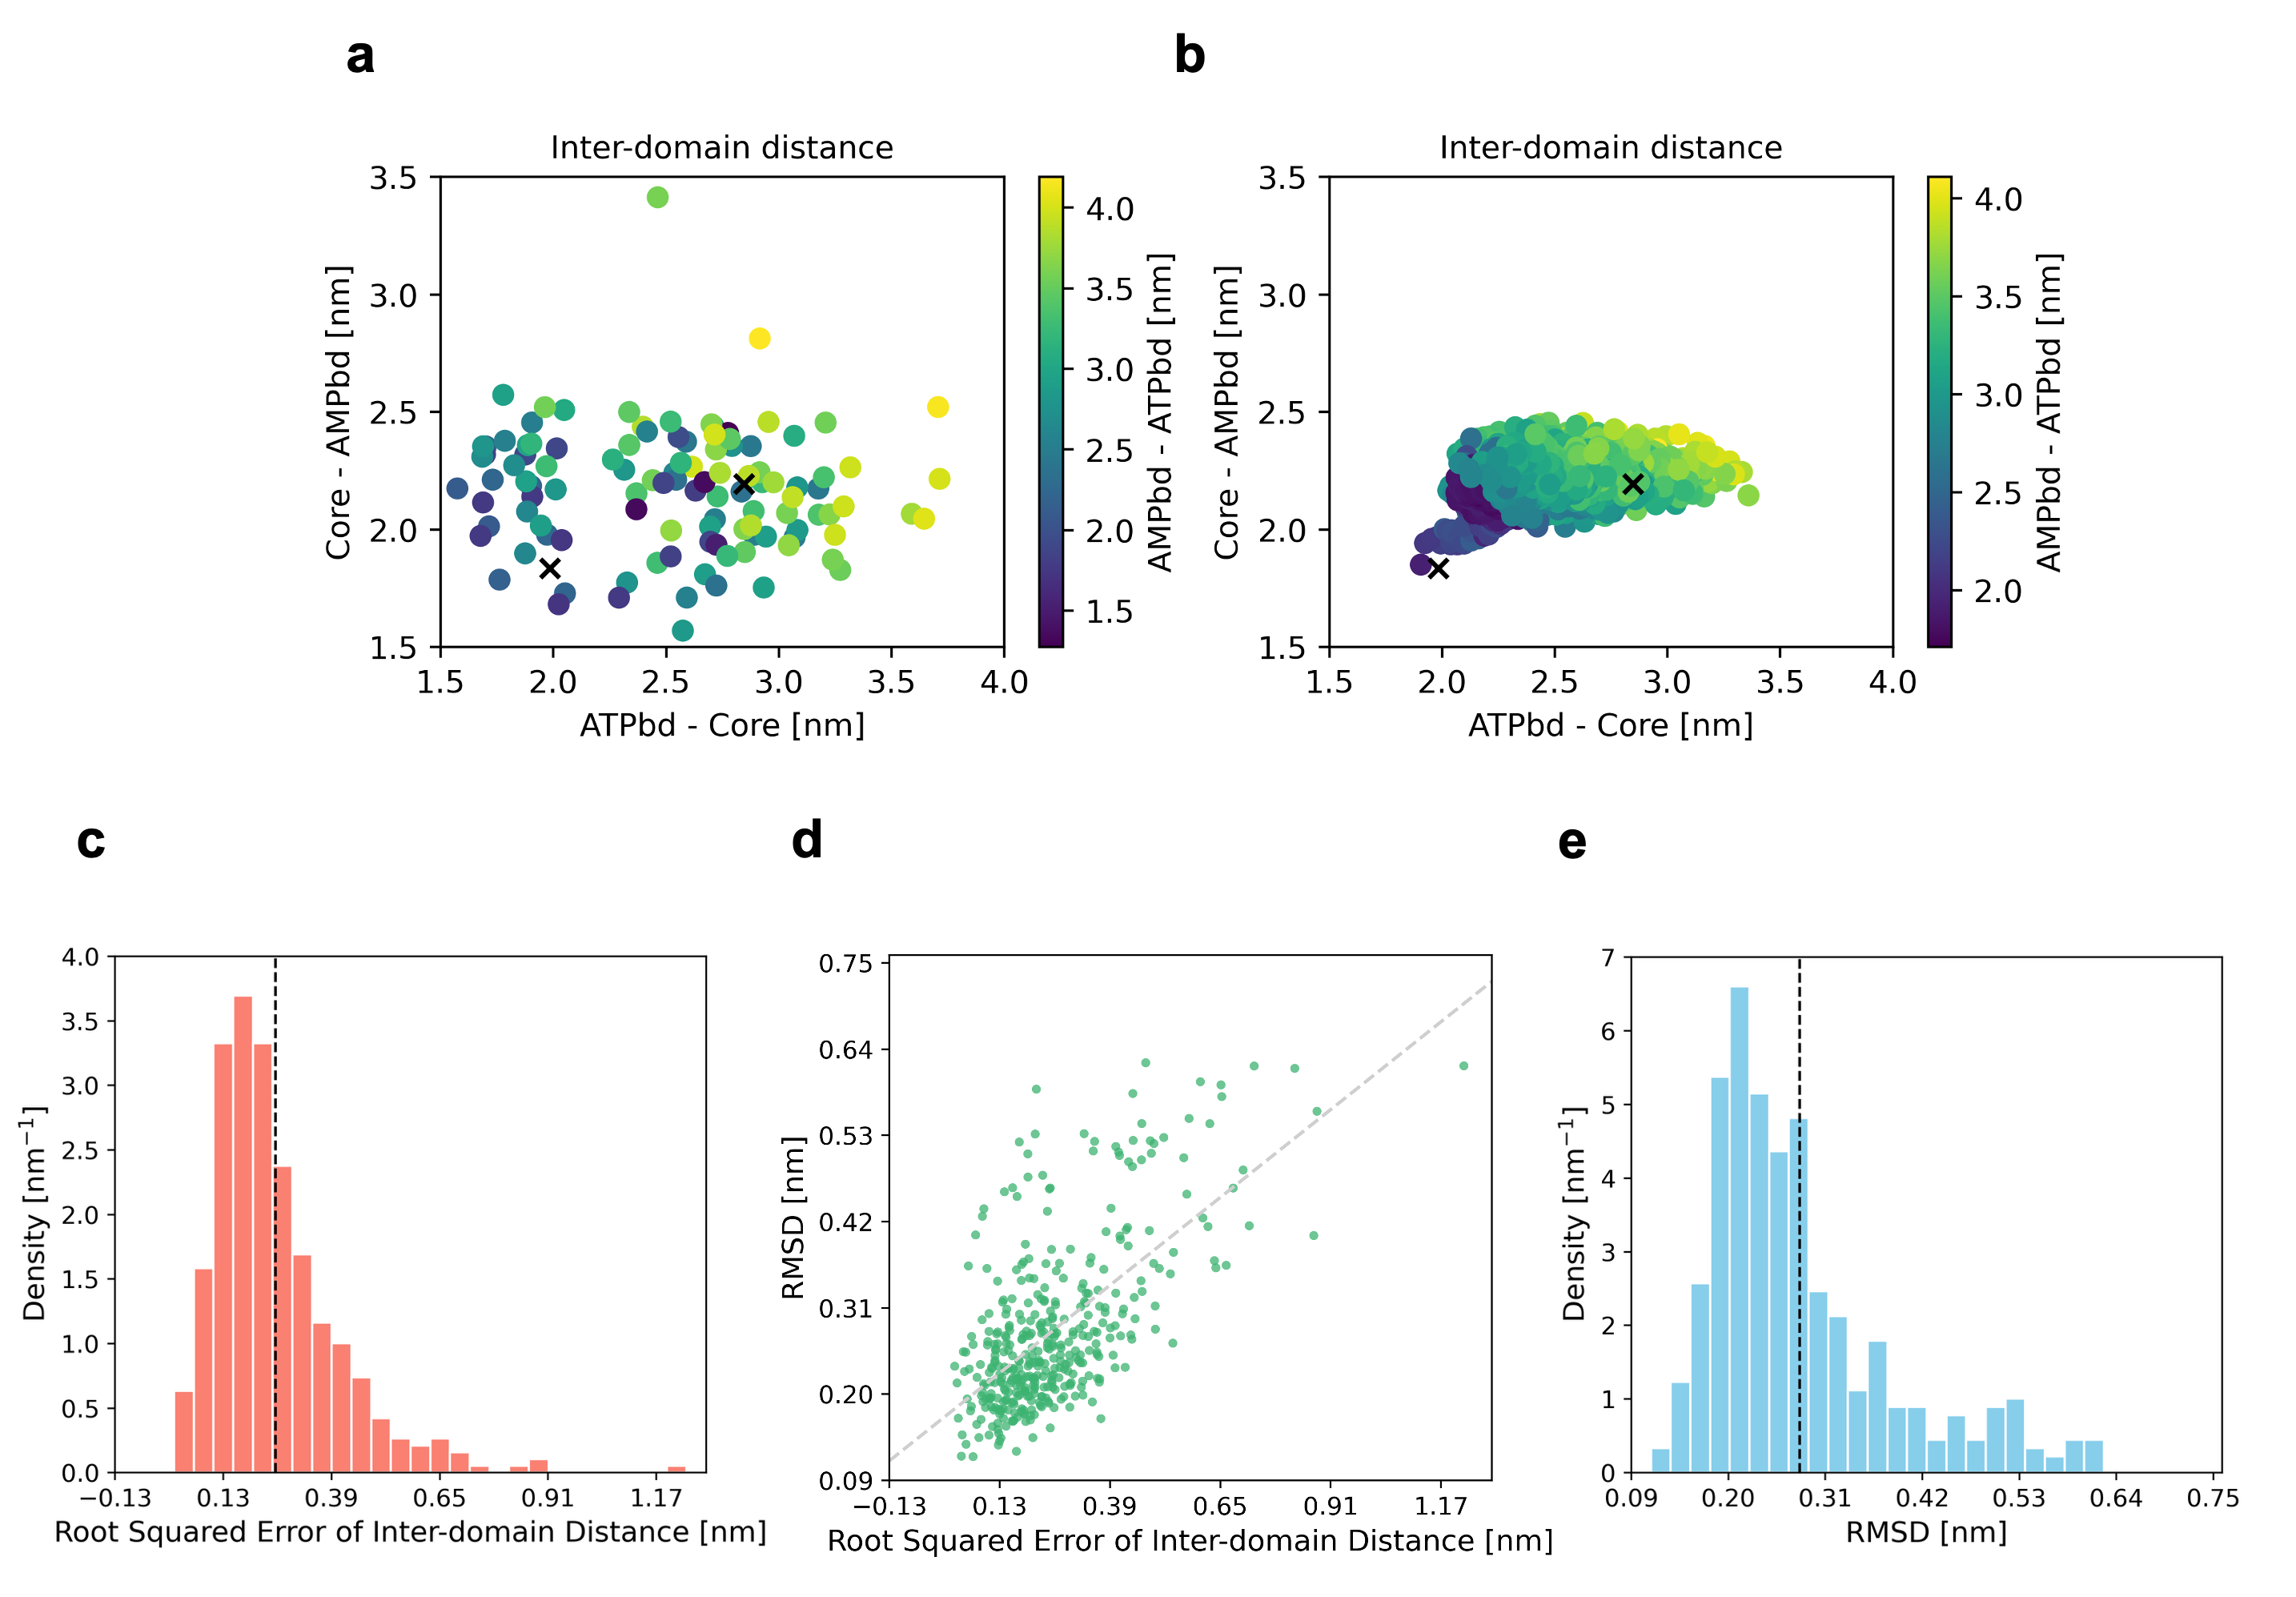
\includegraphics[width=0.75\linewidth]{images/figure-2.png}
    \caption{
        \textbf{Training data and estimation accuracy of \Model}.
        \textbf{(a)} Projection of training data into the inter-domain distance space. The two cross marks represent the open (4AKE) and closed (1AKE) crystal structures from PDB, respectively.
        \textbf{(b)} Projection of a 450 ns MD simulation trajectory into the inter-domain distance space.
        \textbf{(c)} Distribution of the root squared error in the inter-domain distance space between the g-CNN's estimations and the ground-truth. The inter-domain distance was estimated by the trained g-CNN from pseudo-AFM images, which were generated from randomly selected molecular dynamics simulation conformations. The average of the root squared errors is indicated by the broken line (0.254 nm). 
        \textbf{(d)} Scatter plot of the root squared error in the inter-domain distance space and the heavy-atom RMSDs from the ground-truth conformation. 
        The heavy-atom RMSD was computed between the conformation generated with \AFiii navigating using the predicted CV values, and the ground-truth conformation.
        \textbf{(e)} Density of the heavy-atom RMSDs. The average of the RMSD is indicated by the broken line (0.281 nm).
        }
    \label{fig:ak_cnn_training}
\end{figure}

\paragraph{Training data generation and g-CNN accuracy}
We generated a conformational ensemble by navigating \AFiii to target collective variable (CV) values---defined as the inter-domain distances for all domain pairs (LID--CORE, CORE--AMPbd, and AMPbd--LID)---
sampled on a regular grid (see SI section S1 for details of the navigation schedule).
The generated ensembles are shown with their MolProbity scores in \Cref{fig:ak_selection}.
The resulting ensemble adequately covers the broad conformational space of \AK, encompassing both the closed (PDB ID: 1AKE) and open (PDB ID: 4AKE) crystal structures (\Cref{fig:ak_cnn_training}~(a,b)).
We then trained the g-CNN on this ensemble and evaluated its prediction accuracy using pseudo-AFM images generated from randomly selected MD conformations (see \Cref{tab:afm_settings} for the image settings).
The mean root squared error in the CV space is 0.254~nm (\Cref{fig:ak_cnn_training}~(c)), apart from a few outliers exceeding 0.500~nm---sufficiently small to resolve the intermediate conformational states between the open and closed forms of \AK.

\paragraph{Accuracy of conformations estimated by \Model}
We first applied \Model to pseudo-AFM images of the closed and open crystal structures of \AK (\Cref{fig:overview}~(b,c)).
Note that these pseudo-AFM images were generated under idealized imaging conditions (small tip radius, fine resolution, no noise; see Methods), so the accuracy reported here represents an upper bound on what can be achieved; the impact of more realistic conditions is assessed in the robustness analysis below.
The RMSDs between the reconstructed and ground-truth conformations were 0.216~nm (closed) and 0.176~nm (open), both well below the 0.715~nm RMSD separating the two crystal structures, confirming that \Model clearly distinguishes between the two states.
Accordingly, the pseudo-AFM images generated from the estimated conformations are visually similar from the input images, with correlation coefficients (c.c.; \Cref{eq:cc}) of 0.997 (closed) and 0.998 (open).

We next assessed reconstruction accuracy over a broader range of conformations using pseudo-AFM images generated from randomly selected MD snapshots.
Note that these MD conformations span a continuous distribution across the open--closed landscape and are not classified into discrete states; the RMSD and CV errors reported below therefore reflect accuracy over this continuum.
Most RMSDs are distributed around the mean of 0.281~nm, with a small number of outliers (\Cref{fig:ak_cnn_training}~(d,e)).
Inspection of the outlier cases revealed two contributing factors (\Cref{fig:ak_cnn_training}~(d)).
First, depending on how the molecule is oriented on the stage (i.e., which face of the protein contacts the surface), the resulting AFM image may look similar regardless of whether the conformation is open or closed.
Because the g-CNN is trained on pseudo-AFM images rendered from uniformly sampled 3D orientations, it must learn to predict CVs from all possible views; however, certain out-of-plane orientations produce nearly degenerate images for structurally distinct conformations, making it inherently difficult for the g-CNN to estimate the correct inter-domain distances from such views.
Second, even when the predicted CV values are accurate, the reconstructed RMSD can still be elevated because the CV--structure mapping is not unique: 
distinct domain arrangements---such as hinge-bending versus shear-like motions---can yield similar inter-domain distances while producing structurally different conformations.
Indeed, \Cref{fig:ak_cnn_training}~(d) shows that several data points with small CV errors nonetheless exhibit elevated RMSDs, confirming that the CV--structure degeneracy---rather than CV prediction inaccuracy---is the dominant source of reconstruction error in these cases.

\begin{figure}[htbp]
    \centering
    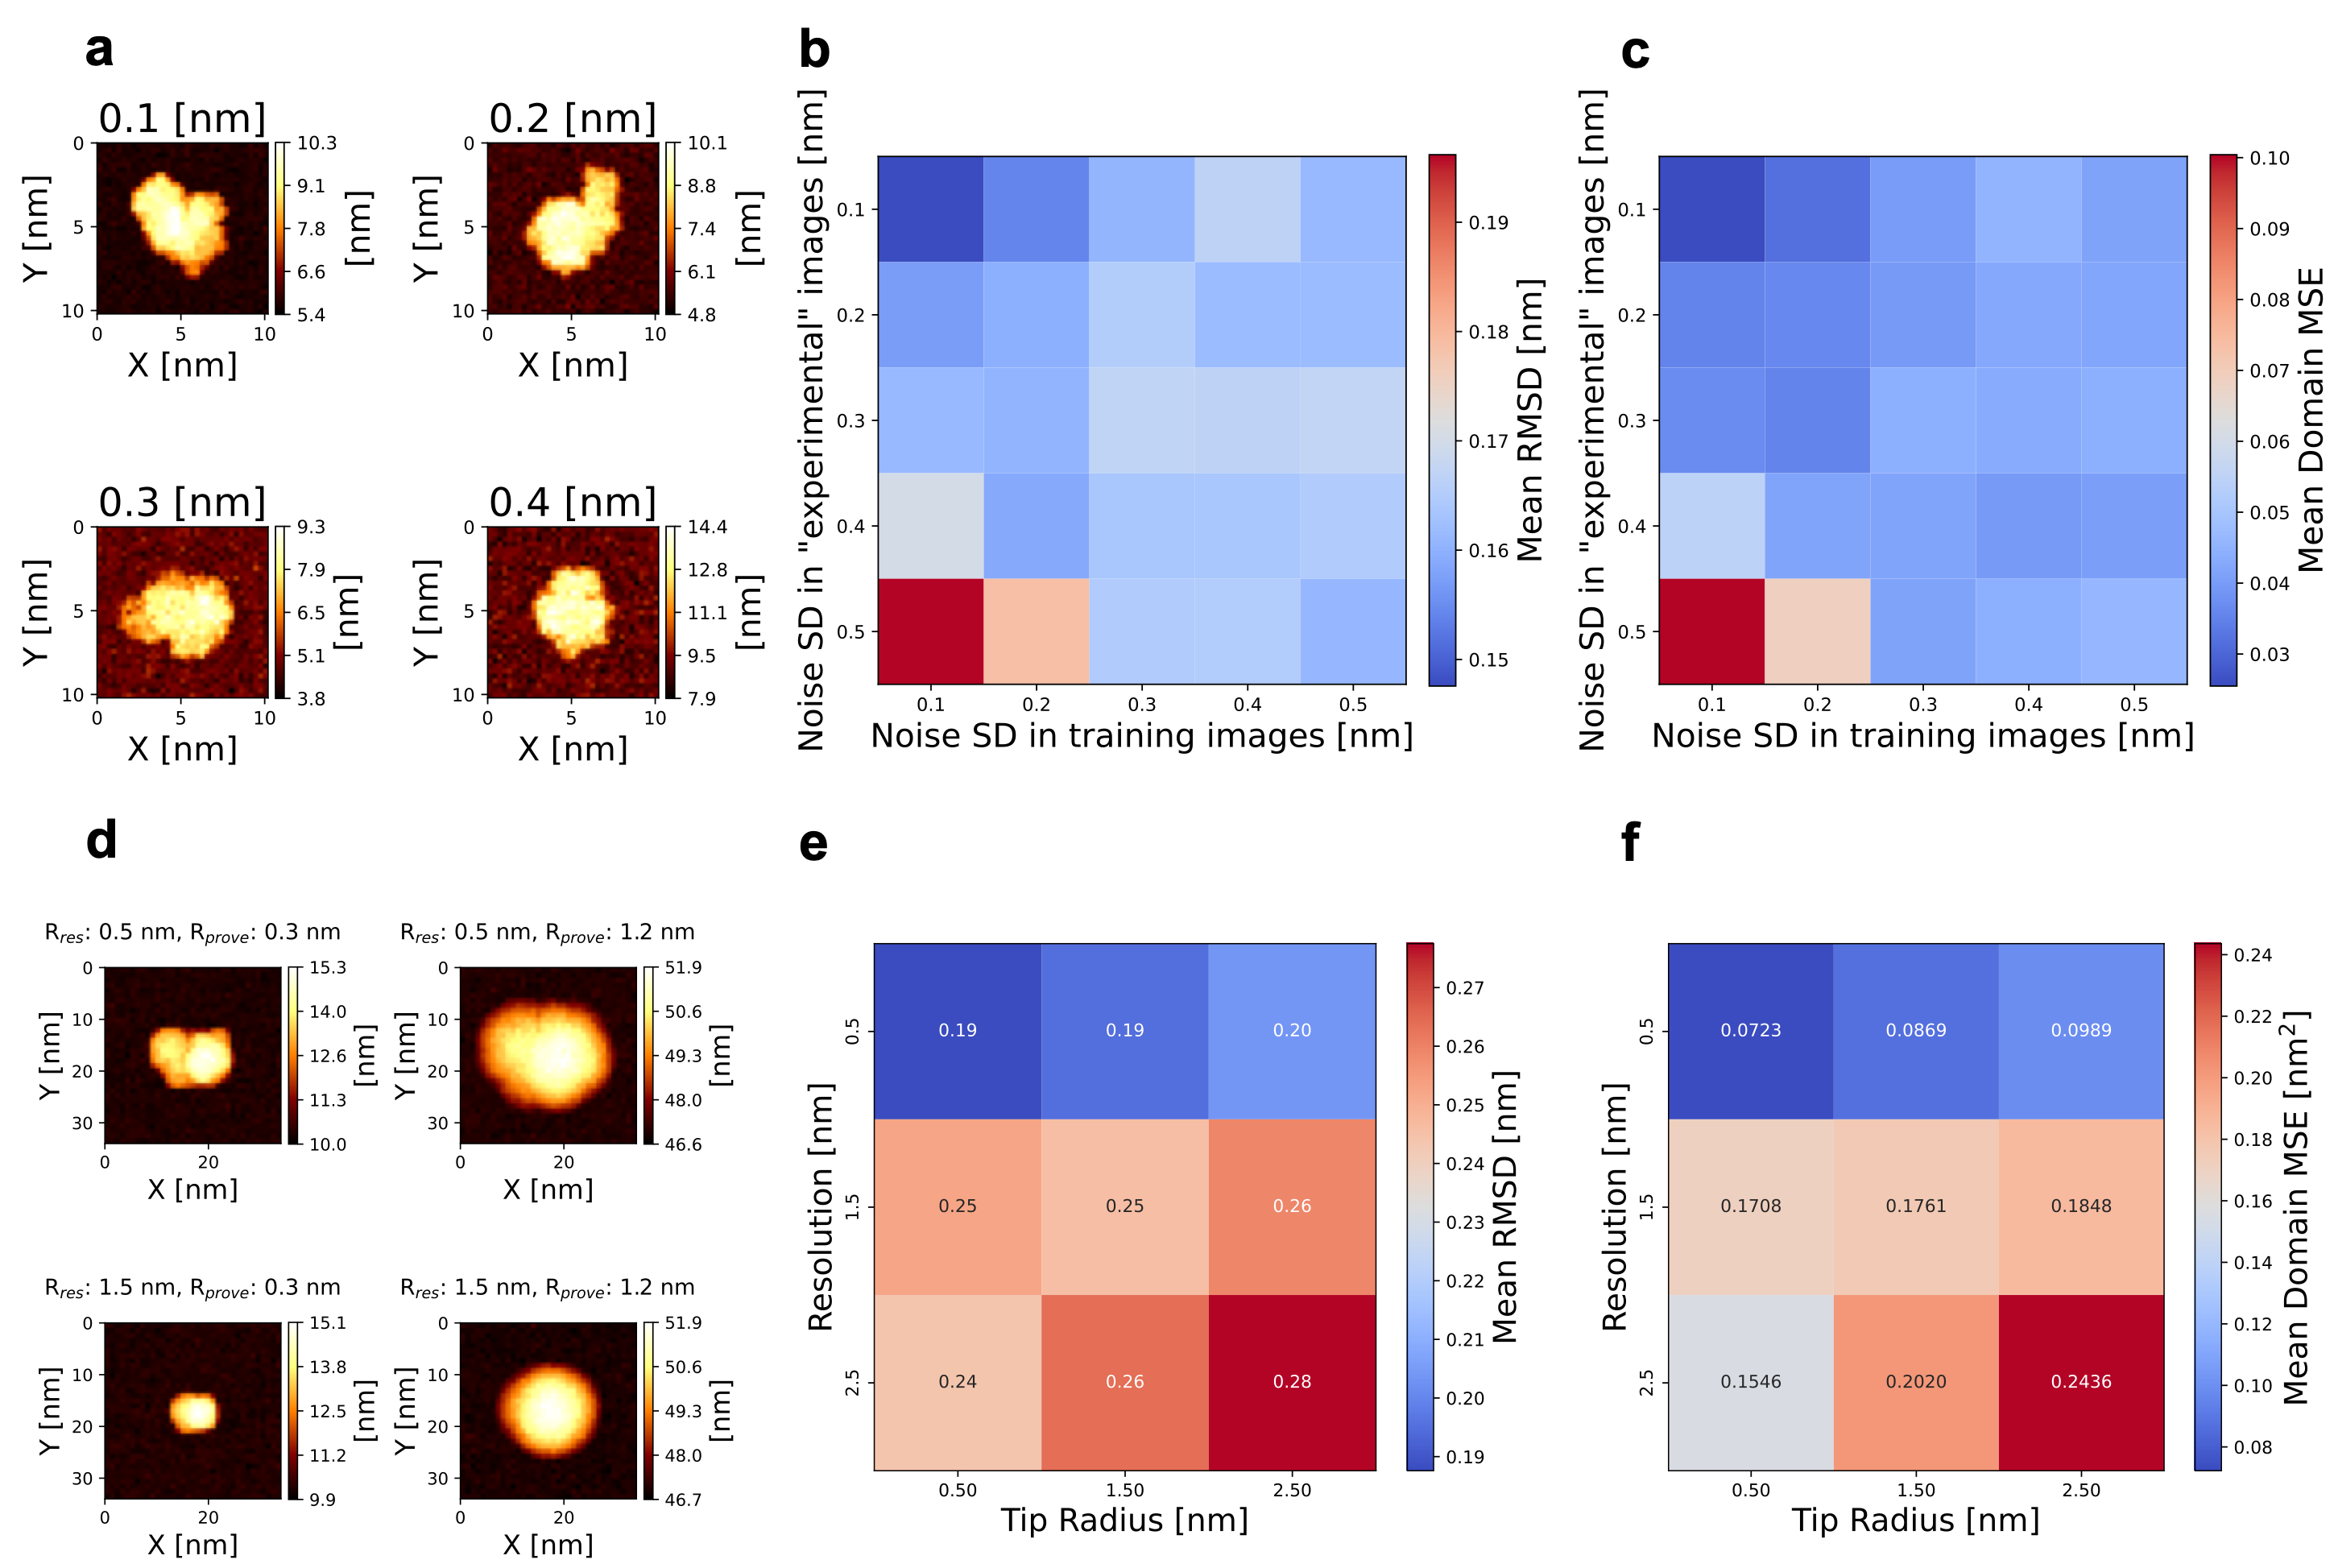
\includegraphics[width=0.75\linewidth]{images/figure-3.png}
    \caption{
        \textbf{Robustness against noise and imaging conditions}.
        \textbf{(a)} Examples of pseudo-AFM images with Gaussian noise at various standard deviations (0.1--0.4~nm), generated from randomly selected MD conformations.
        \textbf{(b)} Mean RMSD between the estimated and ground-truth structures as a function of noise levels in both the training and ``experimental'' pseudo-AFM images. 
        Each value was computed from 20 independent estimations.
        \textbf{(c)} Mean squared error (MSE) of the inter-domain distances under the same noise conditions as in (b).
        \textbf{(d)} Pseudo-AFM images generated with different combinations of the image resolution $R_{\rm res}$ and the probe tip radius $R_{\rm probe}$.
        \textbf{(e)} Mean RMSD between the estimated and ground-truth structures as a function of the tip radius and the image resolution.
        \textbf{(f)} MSE of the inter-domain distances as a function of the tip radius and the image resolution.
    }
    \label{fig:noise_robustness}
\end{figure}

\paragraph{Robustness against noise and imaging conditions}
To evaluate the applicability of \Model to real experimental data, 
we investigated its robustness against two key factors that degrade image quality: 
measurement noise and imaging conditions (image resolution and probe tip radius).

We first examined the effect of noise by systematically varying the Gaussian noise levels added to both the training and ``experimental'' pseudo-AFM images (\Cref{fig:noise_robustness}~(a)).
The resulting heat maps of the mean RMSD (\Cref{fig:noise_robustness}~(b)) and the inter-domain distance MSE (\Cref{fig:noise_robustness}~(c)) reveal two distinct trends.
Adding noise to the ``experimental'' images consistently led to substantial reductions in prediction accuracy, whereas adding noise to the training data alone had a comparatively minor effect; 
indeed, the best performance was achieved with noise-free training data.
These results indicate that \Model is sensitive to noise in the input images but does not require noisy training data to handle noisy inputs.

We next assessed the influence of imaging conditions by varying the image resolution $R_{\rm res}$ and the probe tip radius $R_{\rm probe}$ (\Cref{fig:noise_robustness}~(d)).
The heat maps of the mean RMSD (\Cref{fig:noise_robustness}~(e)) and the inter-domain distance MSE (\Cref{fig:noise_robustness}~(f)) show that image resolution is the dominant factor governing prediction accuracy.
Because \AK is a relatively small molecule, coarse resolution causes it to appear as a nearly featureless round spot, making it difficult for the g-CNN to distinguish different conformations; 
accordingly, degrading the resolution leads to a dramatic increase in estimation error.
In contrast, increasing the probe tip radius has a comparatively modest effect on accuracy, 
indicating that \Model is relatively robust to tip broadening effects.

\paragraph{Correlation coefficient as an evaluation metric}
\begin{figure}[htbp]
    \centering
    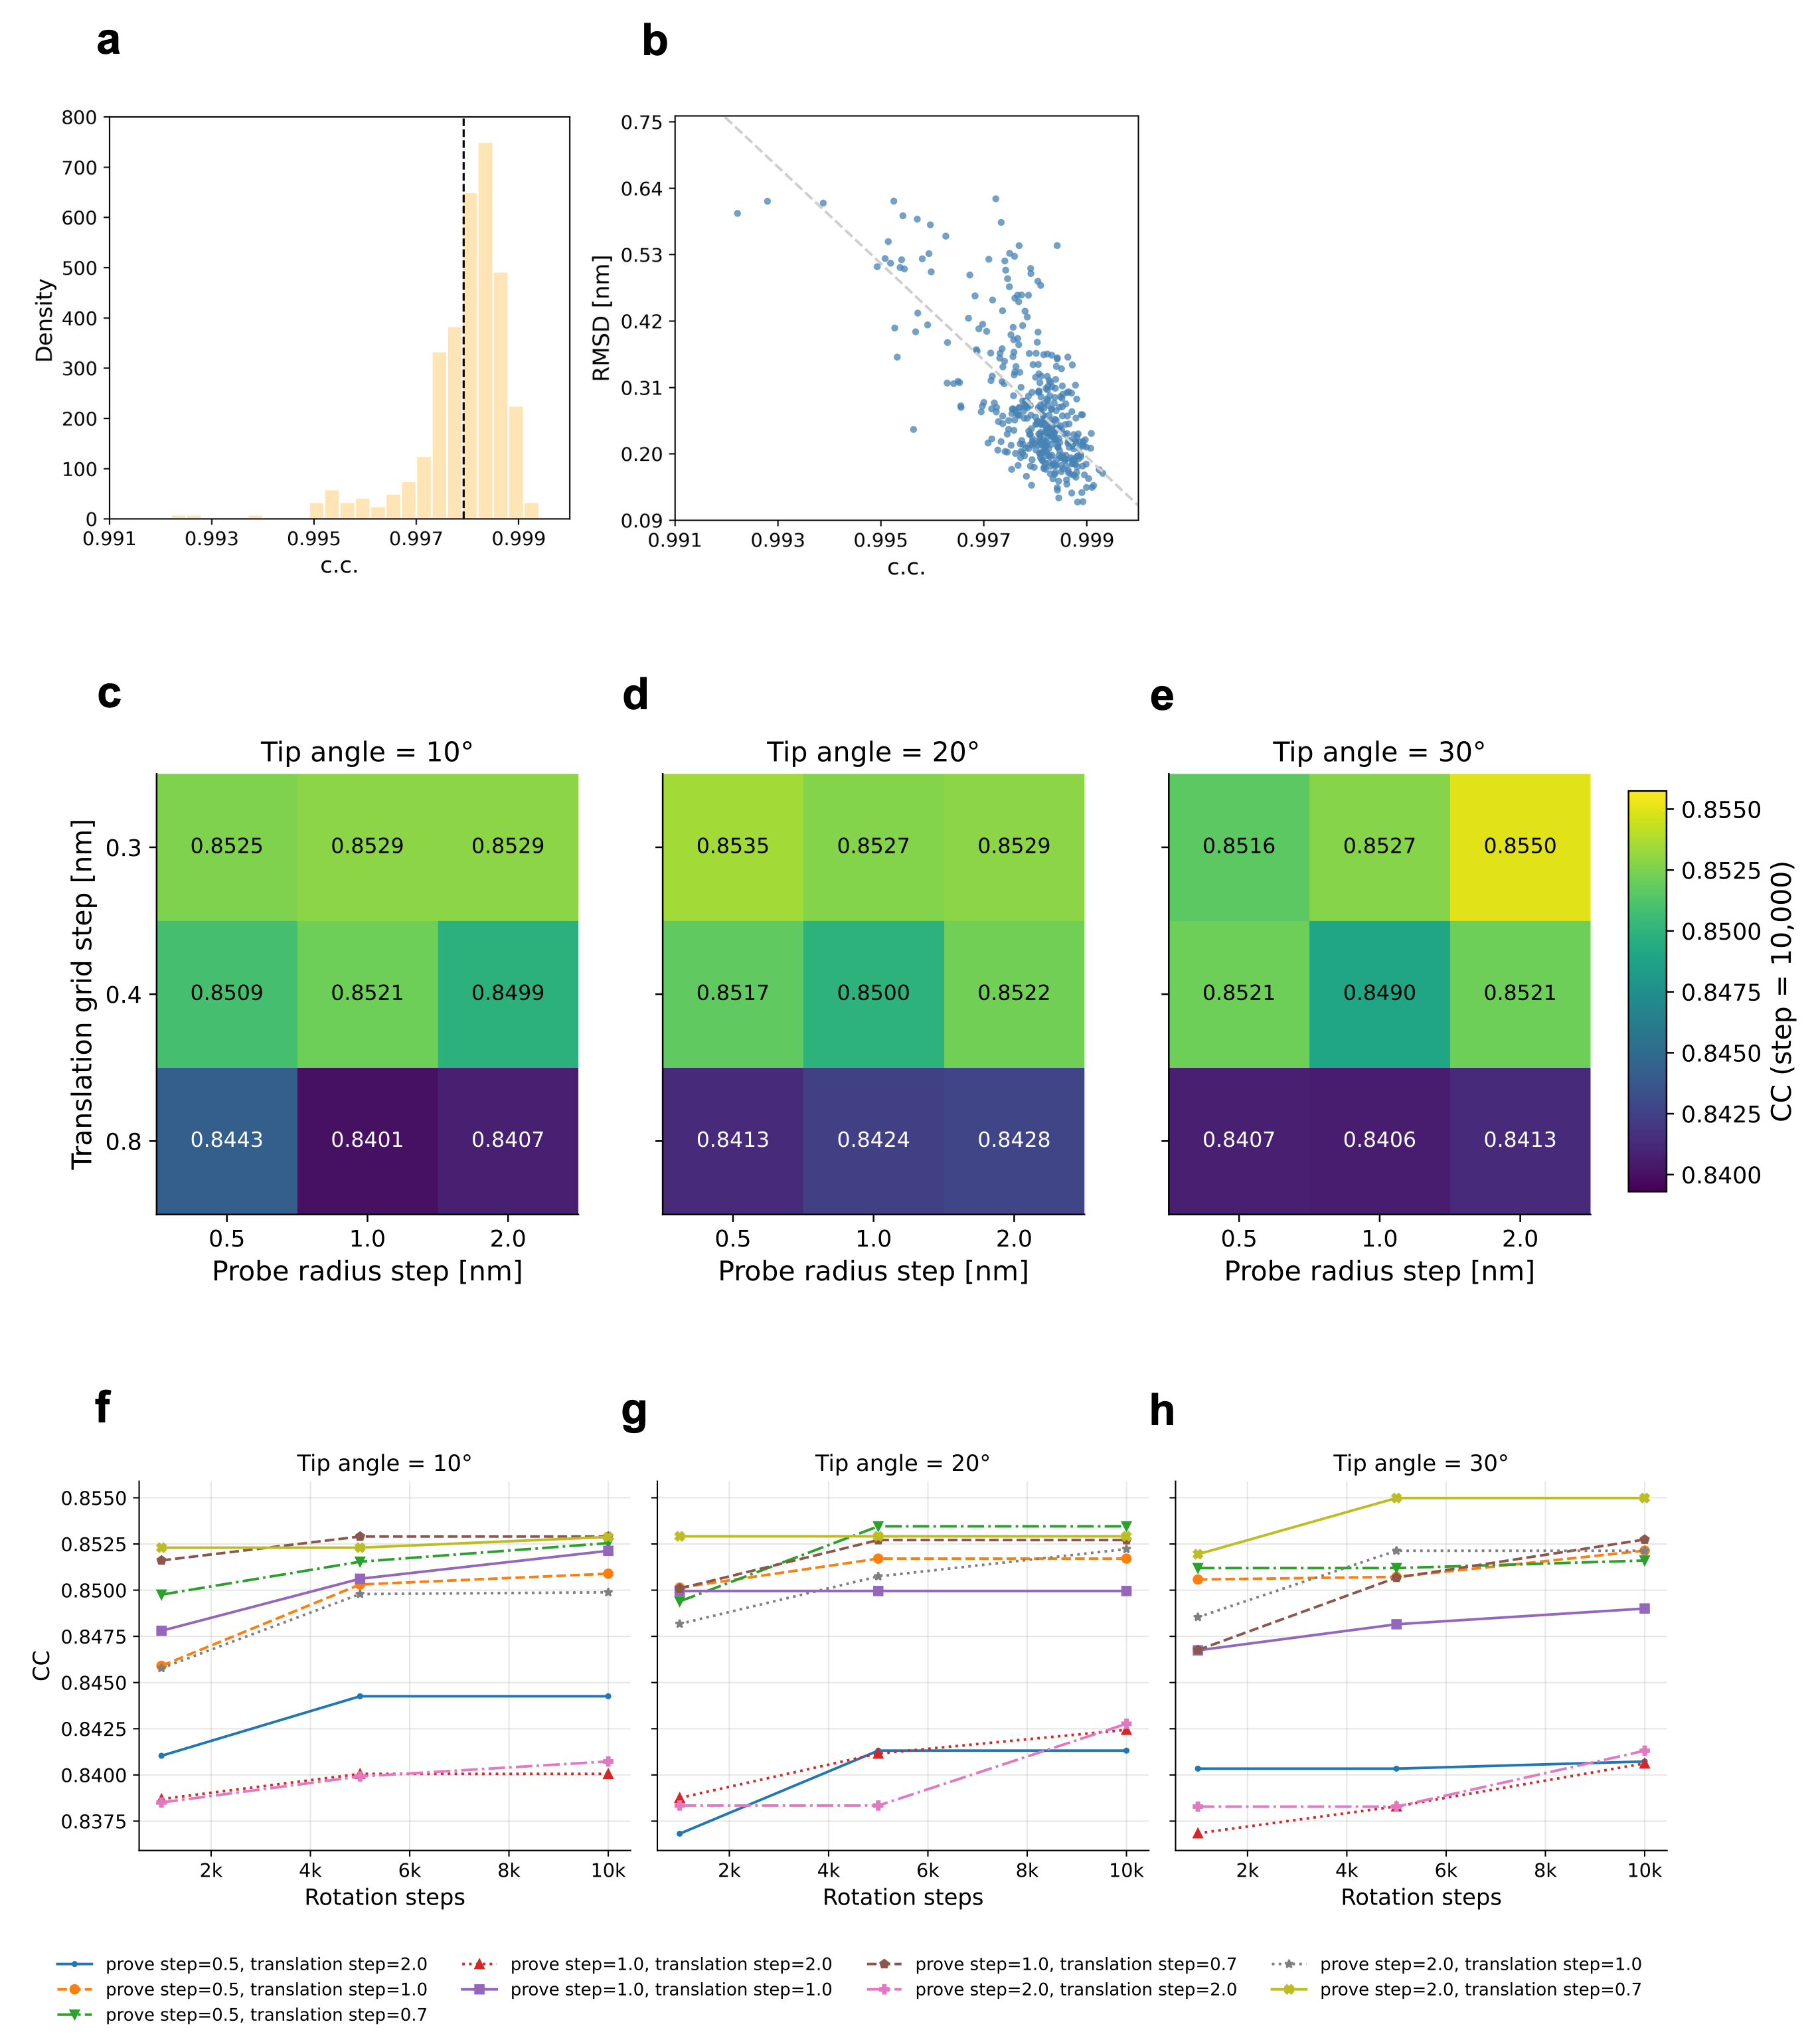
\includegraphics[width=0.75\linewidth]{images/figure-4.png}
    \caption{
        \textbf{Variability of the correlation coefficient and its dependence on fitting parameters}.
        \textbf{(a)} Distribution of correlation coefficients (c.c.) between the ``experimental'' pseudo-AFM images and pseudo-AFM images generated from the estimated conformations after rigid-body fitting. The dashed line indicates the mean value (0.998).
        \textbf{(b)} Scatter plot of the c.c.\ versus the RMSD from the ground-truth conformation. The dashed line shows the linear fit.
        \textbf{(c--e)} Maximum c.c.\ achieved for different combinations of the translation grid step and the probe radius step at tip angles of $10^{\circ}$ (c), $20^{\circ}$ (d), and $30^{\circ}$ (e).
        \textbf{(f--h)} Maximum c.c.\ as a function of the number of rotation search steps at tip angles of $10^{\circ}$ (f), $20^{\circ}$ (g), and $30^{\circ}$ (h). Different curves correspond to different combinations of the probe radius step and translation grid step.
    }
    \label{fig:cc}
\end{figure}

When applying \Model to real experimental data, ground-truth structures are unavailable and RMSD cannot be computed. 
We therefore examined whether the correlation coefficient (c.c.) between pseudo-AFM images and the reference images can serve as a reliable proxy for structural accuracy.

The c.c.\ values are concentrated in a narrow range of 0.995--0.999, with a mean of 0.998 (\Cref{fig:cc}~(a)). 
Despite this narrow distribution, a clear negative correlation exists between the c.c.\ and the RMSD (\Cref{fig:cc}~(b)), confirming that the c.c.\ is indeed a meaningful indicator of structural agreement. 
Notably, however, even a modest difference of $\sim$0.01 in c.c.\ can correspond to a wide range of RMSD values (\Cref{fig:cc}~(b)), implying that small improvements in c.c.\ often reflect substantial differences in structural accuracy. 
This observation underscores the importance of precise c.c.\ evaluation: the metric is reliable, but the structurally relevant signal resides in very small numerical differences.

We next investigated how sensitively the c.c.\ depends on the parameters of the rigid-body fitting procedure. 
Using a single experimental AFM image and the crystal structure of \flhac (discussed in the next section) as the target, we performed repeated fitting trials in which the structure was randomly rotated and then optimized over translation and probe tip radius at various grid step sizes (\Cref{fig:cc}~(c--e)). 
The c.c.\ was highly sensitive to the translation grid step: a coarse translation search frequently failed to locate the optimal c.c.\ value. 
In contrast, the c.c.\ was relatively insensitive to the probe radius grid step. 
For the rotational search, the c.c.\ converged in most cases by approximately 5,000 rotation steps (\Cref{fig:cc}~(f--h)). 
Based on these results, we adopted a translation step of 0.7~nm, a probe radius step of 1~nm (2~nm -- 6~nm for \flhac), a tip angle of $20^{\circ}$, and 10,000 rotation steps for all subsequent analyses, which we consider sufficient for reliable c.c.\ evaluation.
With these settings, the rigid-body fitting takes approximately 3 minutes per structure on a single GPU.

\subsection{Application to real experimental AFM images: a flagellar protein \flhac}

FlhA is a key component of the flagellar protein export system, and its C-terminal domain, \flhac, helps transport proteins by assisting their binding to the exporter. 
Structurally, it comprises four domains (\acdi, \acdii, \acdiii, and \acdiv) and a linker to the transmembrane domain (FlhA\textsubscript{TM}) (\Cref{fig:flhac_results}~(a)). 
Previous studies using X-ray crystallography and mutational analysis indicate that hinge motions among these domains influence transport activity and motility \cite{saijo-hamano2010flha}. 
%Here, we applied \Model to real experimental AFM images of \flhac to evaluate its ability to reconstruct the 3D structure of \flhac from AFM images. 

Here, to evaluate the applicability of \Model to real AFM data, we used HS-AFM images of \flhac acquired by Inoue et al.\ \cite{inoue_structural_2019}.
The images were recorded with a spatial resolution of approximately 1.0~nm/pixel (59 $\times$ 59~nm$^2$ field of view, 60 $\times$ 60 pixels) and a frame interval of 66~ms, with the sample immobilized on mica in a buffer containing 20~mM NaCl and 10~mM Tris-HCl (pH~8.0).
We estimated the conformations of \flhac using \Model from 159 HS-AFM images of the \flhac monomer.
It should be noted that, whereas conventional flexible fitting methods for capturing structural changes typically require hours to days of computation per AFM image even with a coarse-grained model \cite{Niina2020},
\Model allows estimation of conformations from each AFM image in approximately one minute on a single GPU once the g-CNN has been trained (see Conclusion for a discussion of the training cost).
This enabled, for the first time, the processing of as many as 159 AFM images in this study.

\paragraph{Training of the g-CNN and ResNet-18}
Conformations for training the g-CNN were generated by navigating \AFiii with CV values on a grid as described in \textit{Training}. 
As the CVs, we used the inter-domain distances of domain pairs, \acdi--\acdiv, \acdii--\acdiii, and \acdii--\acdiv. 
The generated ensembles are shown with their MolProbity scores in \Cref{fig:flhac_selection}. 
The g-CNN was trained on the training data to learn the relationship between AFM images and the CVs.

We also trained ResNet-18 on the combination of the g-CNN's training images and the experimental AFM images 
to obtain embedding representations that capture the molecular features in AFM images.
To verify that the learned embeddings encode structurally meaningful information, 
we projected the 256-dimensional embedding vectors onto two dimensions using UMAP \cite{mcinnes2018umap} (\Cref{fig:resnet_embeddings}~(a--c)). 
The resulting scatter plots, colored by each of the three inter-domain distances, show that different inter-domain distances correspond to distinct directions in the embedding space, 
indicating that the embeddings successfully capture conformational variations.
We further confirmed that the embeddings are approximately invariant to in-plane rotation of the molecule.
For each of 20 randomly selected conformations, we generated pseudo-AFM images at $15^{\circ}$ rotation increments and computed their pairwise distances in the embedding space (\Cref{fig:resnet_embeddings}~(d)).
The cosine similarity between embeddings of rotationally related images was consistently high (mean = 0.948; \Cref{fig:resnet_embeddings}~(e)), 
and the L2 distance was consistently low (mean = 0.179; \Cref{fig:resnet_embeddings}~(f)), 
both well separated from the distributions of randomly sampled pairs.
These results, together with visual inspection, support the use of the embedding distance as a measure of image similarity: 
images that are close in the embedding space can be regarded as depicting similar molecular shapes.

\begin{figure}[htbp]
    \centering
    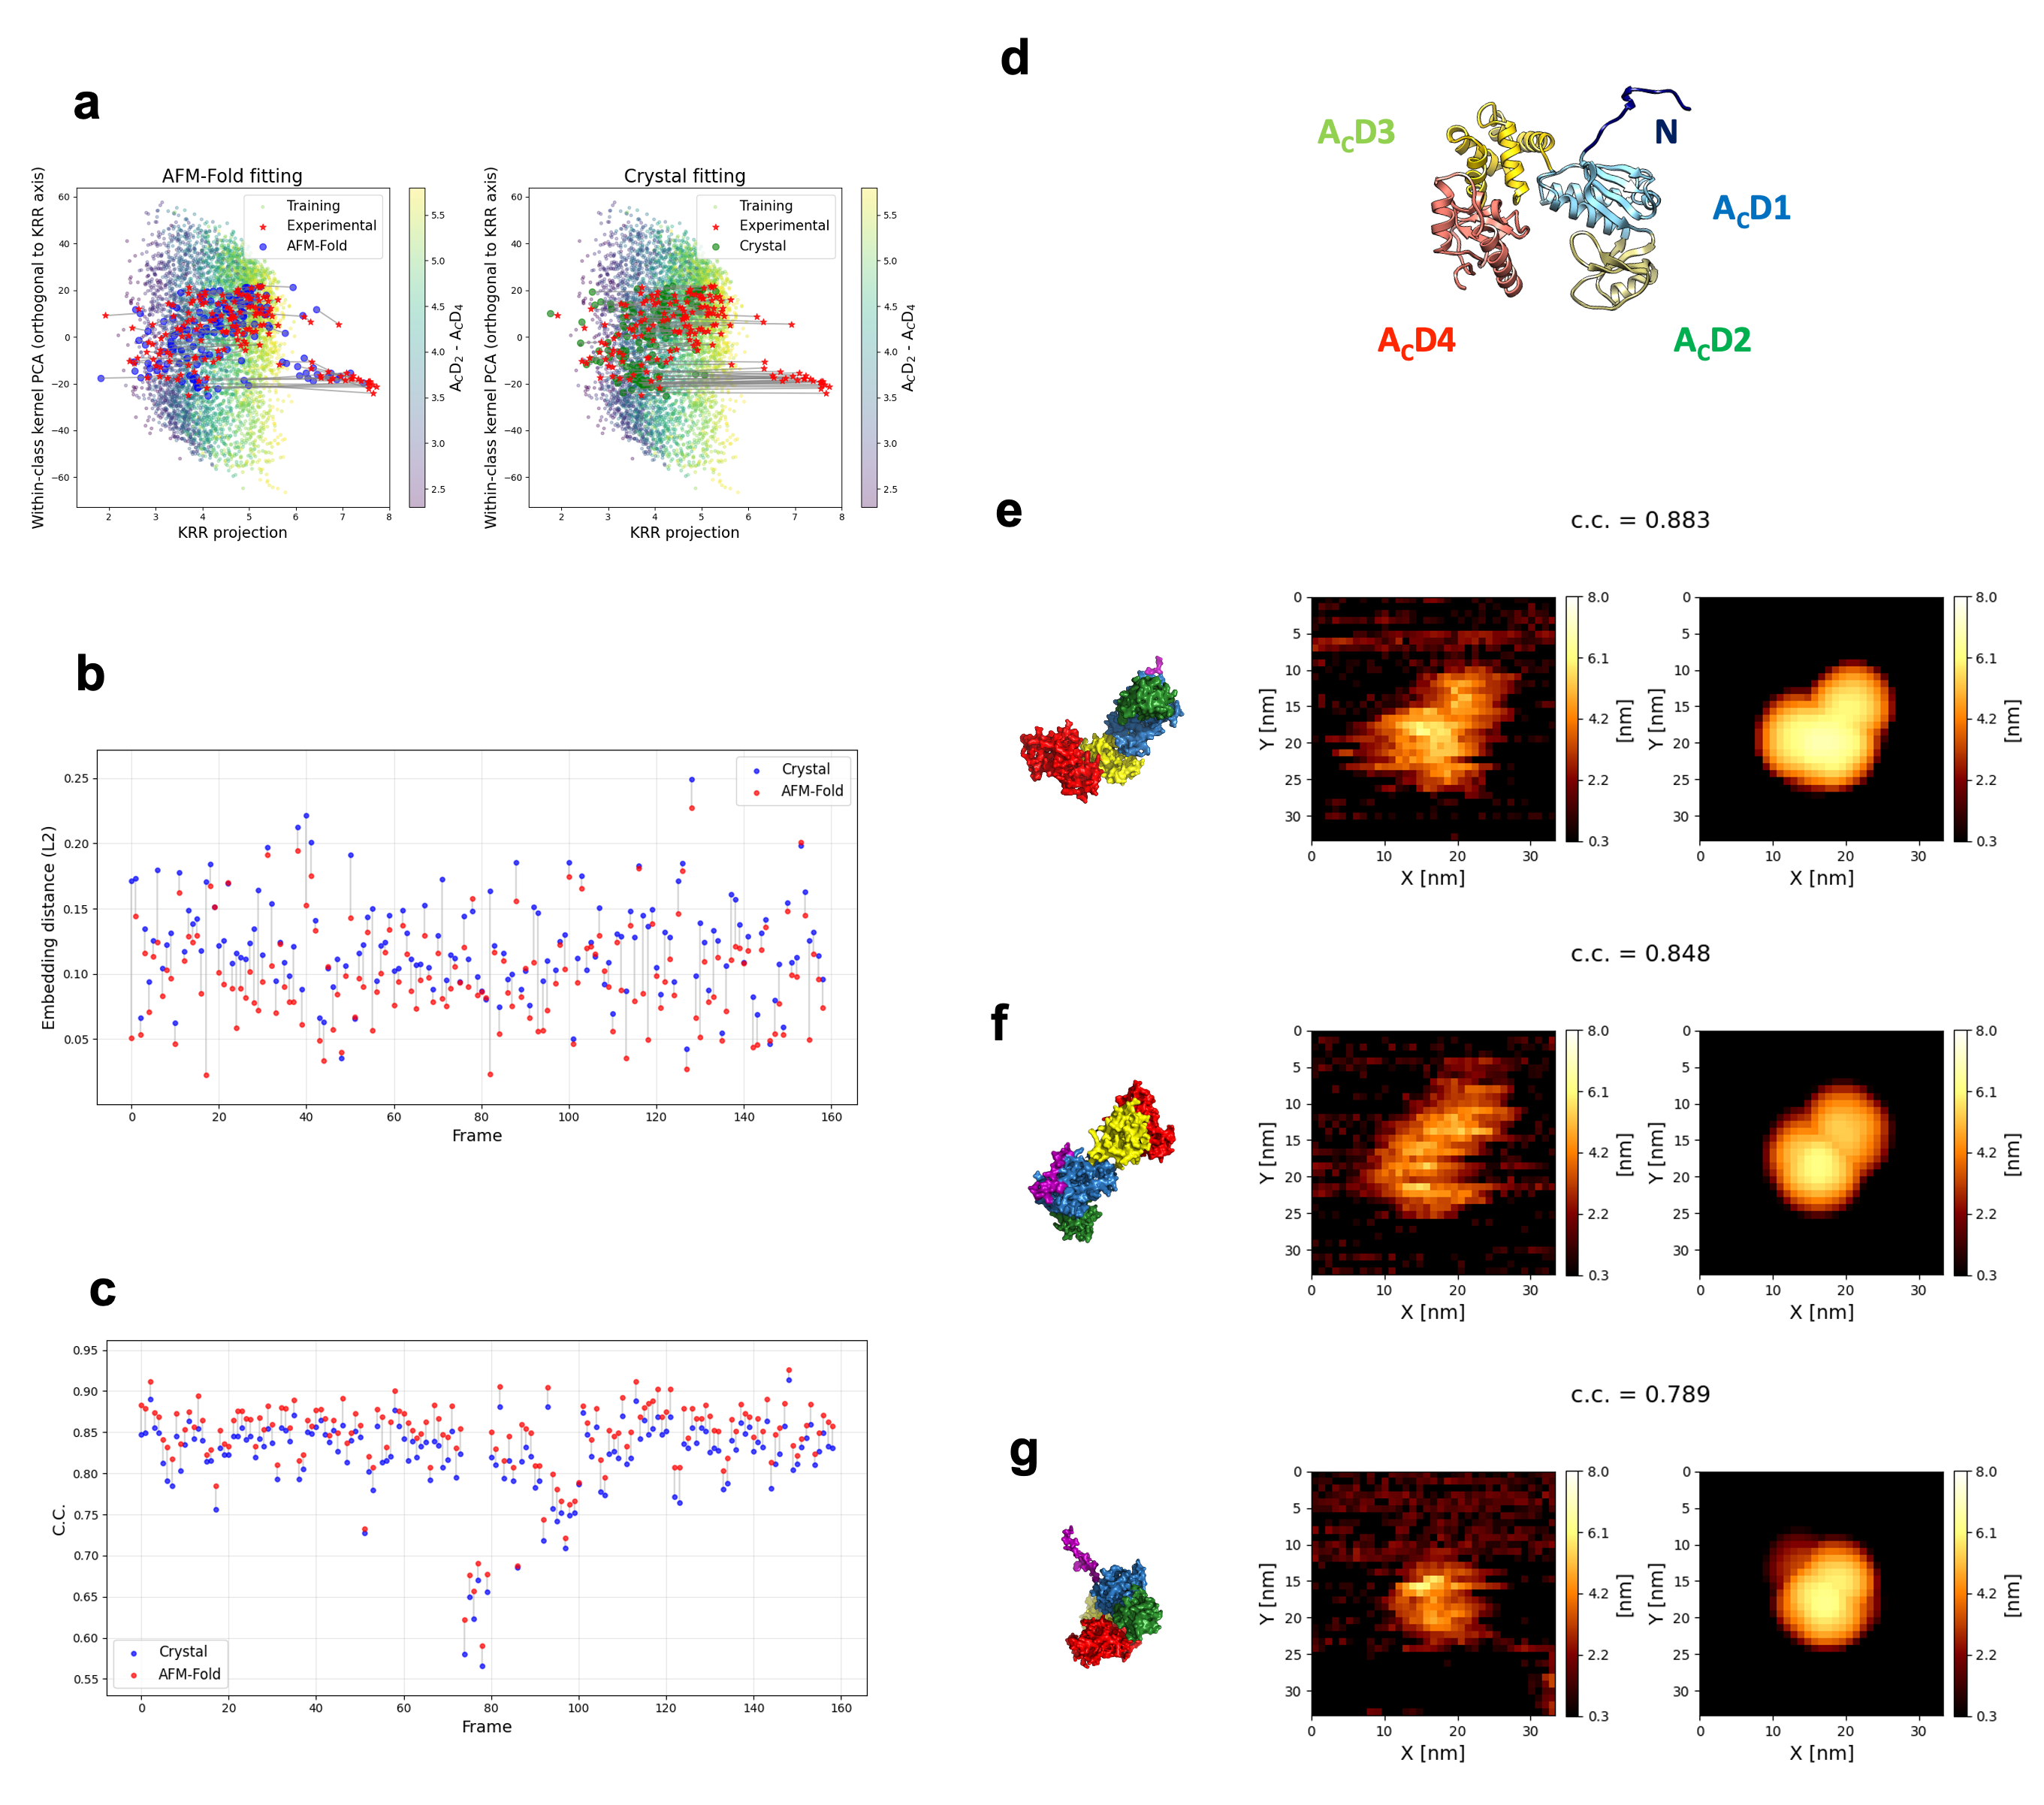
\includegraphics[width=0.75\linewidth]{images/figure-5.png}
    \caption{
        \textbf{Embedding representations learned by ResNet-18}.
        \textbf{(a--c)} UMAP projections of the 256-dimensional ResNet-18 embeddings for the training pseudo-AFM images and the experimental AFM images (red). Each scatter plot is colored by a different inter-domain distance: \acdii--\acdiv (a), \acdii--\acdiii (b), and \acdi--\acdiv (c). Different inter-domain distances correspond to distinct gradient directions in the embedding space.
        \textbf{(d)} Representative pseudo-AFM images of a single conformation rotated in the image plane at $15^{\circ}$ increments. Twenty such sets were prepared for statistical evaluation.
        \textbf{(e)} Distribution of cosine similarity in the embedding space. The gray histogram shows the distribution for randomly sampled image pairs from the training data. The blue dashed line indicates the mean cosine similarity for rotationally related image pairs (0.948), which remains high even when the variance is taken into account.
        \textbf{(f)} Distribution of L2 distance in the embedding space. The gray histogram shows the distribution for randomly sampled pairs. The green dashed line indicates the mean L2 distance for rotationally related pairs (0.179), which remains low even when the variance is taken into account.
    }
    \label{fig:resnet_embeddings}
\end{figure}

\paragraph{Evaluating estimated conformations by \Model}
We applied \Model to all 159 experimental AFM images and quantified the agreement between each estimated (or crystal) structure and the corresponding experimental image using two complementary metrics: 
the correlation coefficient (c.c.) and the L2 distance in the ResNet-18 embedding space. 
For each metric, we searched for the rendering pose that maximizes the similarity to the experimental image.

Both metrics consistently showed that \Model estimations agree with the experimental images better than the crystal structure.
In the embedding-space evaluation, the \Model estimations achieved smaller L2 distances than the crystal structure for the majority of frames (\Cref{fig:flhac_results}~(i)), with most distances falling below 0.3---within the rotational invariance range established in \Cref{fig:resnet_embeddings}~(f)---confirming that the generated images share similar shape features with the experimental data.
Likewise, in the c.c.-based evaluation, \Model achieved higher c.c.\ values in the majority of cases (\Cref{fig:flhac_results}~(j)).
\Cref{fig:flhac_results}~(b--f) illustrates a case in which the crystal structure clearly fails to reproduce the experimental image, whereas the \Model estimation captures the observed features in both the L2-based (\Cref{fig:flhac_results}~(c,d)) and c.c.-based (\Cref{fig:flhac_results}~(e,f)) fittings.

It should be noted, however, that the numerical margins are modest in both metrics. This reflects an intrinsic degeneracy in AFM imaging: distinct 3D conformations can yield similar AFM images due to the convolution effects of the probe tip, finite resolution, and measurement noise.
Indeed, although the embedding space analysis revealed that experimental images are predominantly surrounded by open conformations (\Cref{fig:flhac_results}~(g)), the closed crystal structure was still able to produce pseudo-AFM images of comparable similarity (\Cref{fig:flhac_results}~(h)), because under realistic imaging conditions, even a closed conformation can mimic the appearance of an open one.
Moreover, the c.c.\ is dominated by the overall molecular envelope and is inherently insensitive to fine internal structural rearrangements, as demonstrated for \AK (\Cref{fig:cc}~(a)); consequently, even meaningful conformational differences manifest as only small numerical changes in c.c.\ values.
Nevertheless, the fact that \Model consistently outperforms the crystal structure across both metrics and the majority of frames supports the conclusion that it captures genuine conformational features present in the experimental AFM images.

\begin{figure}[htbp]
    \centering
    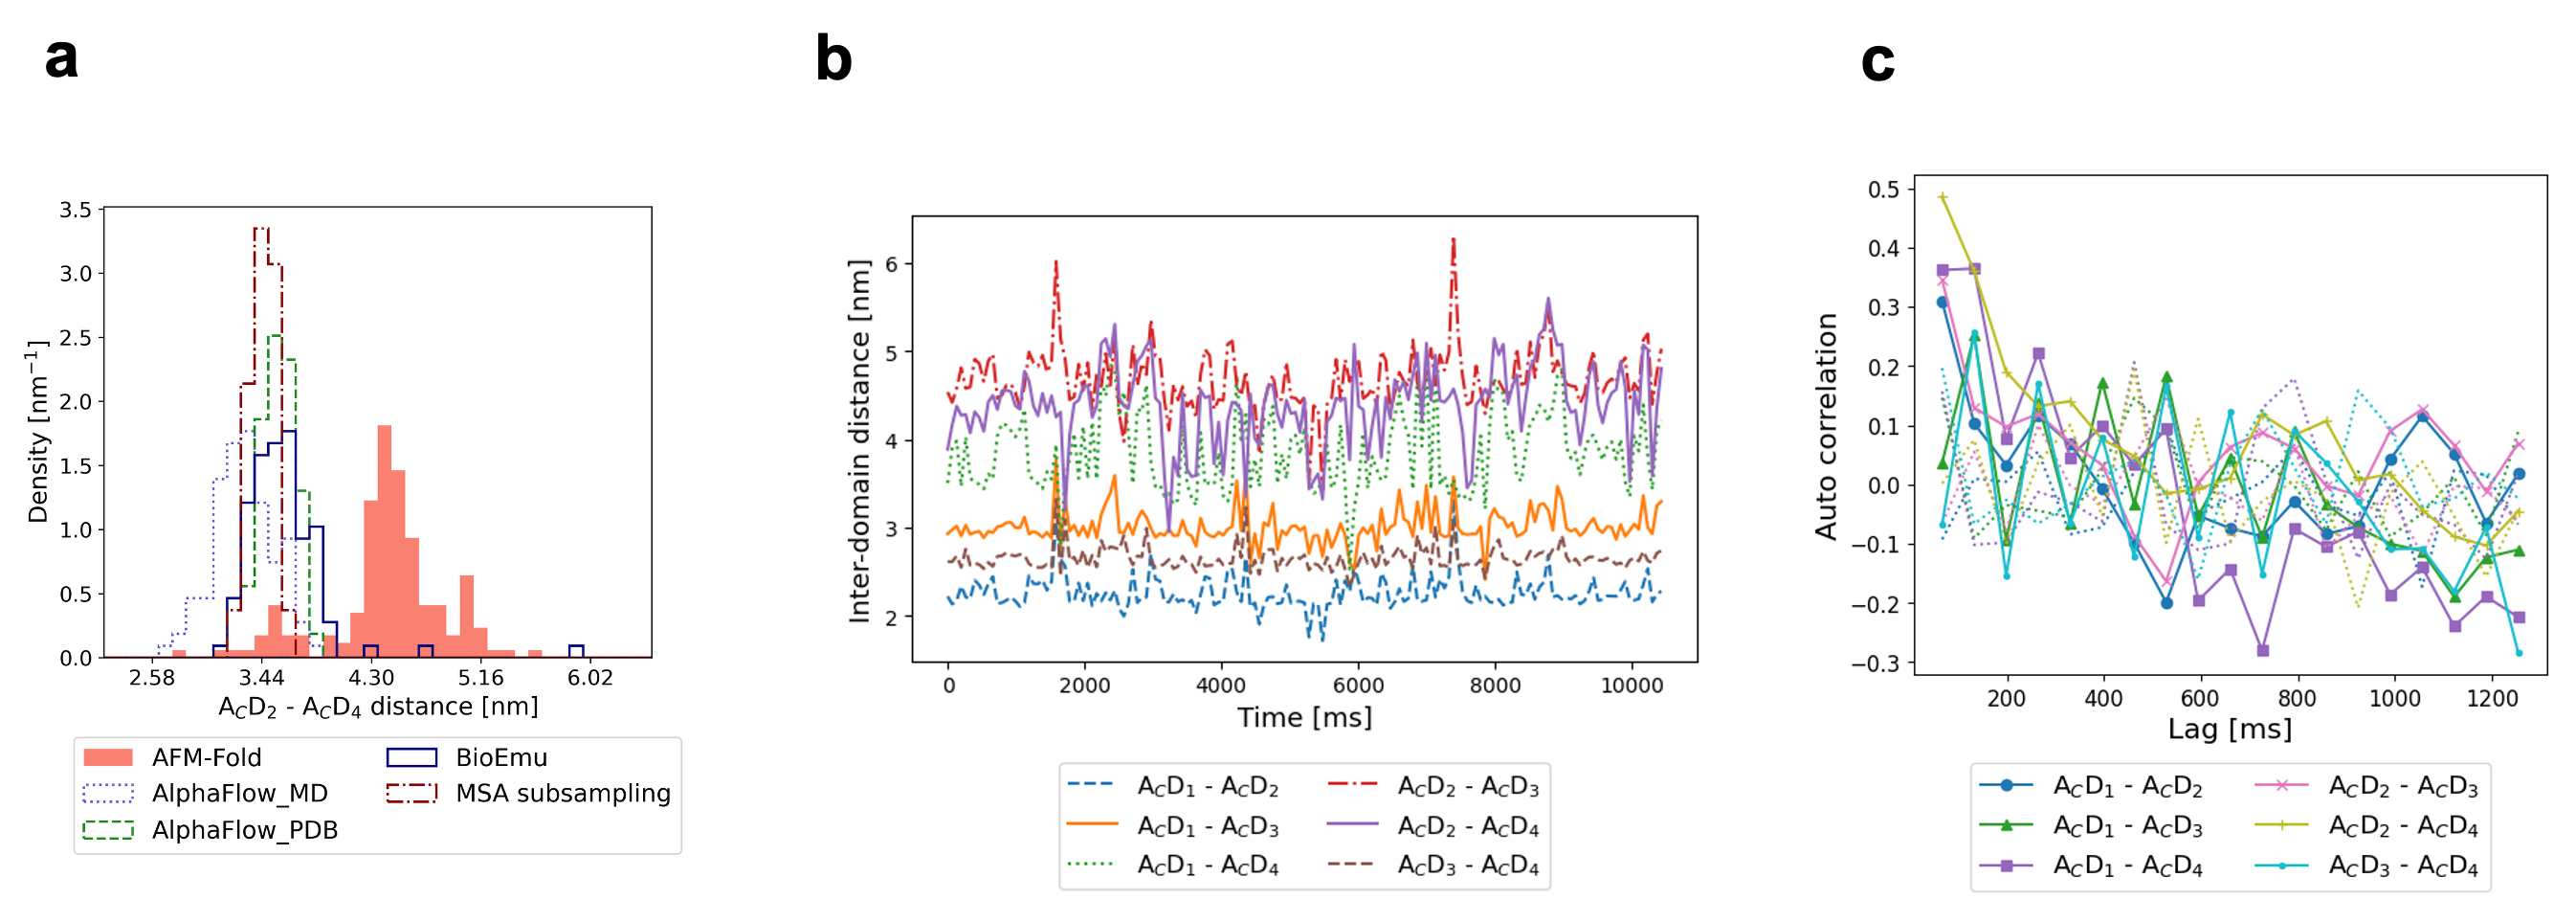
\includegraphics[width=0.75\linewidth]{images/figure-6.png}
    \caption{
        \textbf{Comparison of \Model estimations and the crystal structure for \flhac}.
        \textbf{(a)} Crystal structure of \flhac (PDB ID: 3A5I). The four domains are colored as follows: dark blue, linker; sky blue, \acdi; green, \acdii; yellow, \acdiii; and orange, \acdiv.
        \textbf{(b)} A representative experimental AFM image in which the crystal structure poorly reproduces the observed features.
        \textbf{(c,d)} Pseudo-AFM images generated from the crystal structure (c) and the \Model estimation (d) after rigid-body fitting based on the L2 distance in the embedding space. Predicted domain positions are overlaid.
        \textbf{(e,f)} Pseudo-AFM images generated from the crystal structure (e) and the \Model estimation (f) after rigid-body fitting based on the c.c.\ value. Predicted domain positions are overlaid.
        \textbf{(g,h)} UMAP projections of the ResNet-18 embeddings, showing the positions of the fitted pseudo-AFM images (blue in (g), green in (h)) relative to the training data (gray) and experimental images (red), for the \Model estimations (g) and the crystal structure (h).
        \textbf{(i)} Scatter plot comparing the L2 distances from the experimental image to the \Model estimation ($y$-axis) and to the crystal structure ($x$-axis). Points below the diagonal indicate cases where \Model achieves a closer match. Marginal histograms on the top and right axes show the distributions of L2 distances for the crystal structure and \Model, respectively.
        \textbf{(j)} Bland--Altman plot of the c.c.\ values. The $x$-axis shows the mean of $\mathrm{c.c._{AFMFold}}$ and $\mathrm{c.c._{Crystal}}$, and the $y$-axis shows their difference. Points are colored by the \acdii--\acdiv inter-domain distance. The dashed line indicates the mean difference. The marginal histogram on the right shows the distribution of c.c.\ differences (improvement of \Model over the crystal structure).
    }
    \label{fig:flhac_results}
\end{figure}


\begin{figure}[htbp]
    \centering
    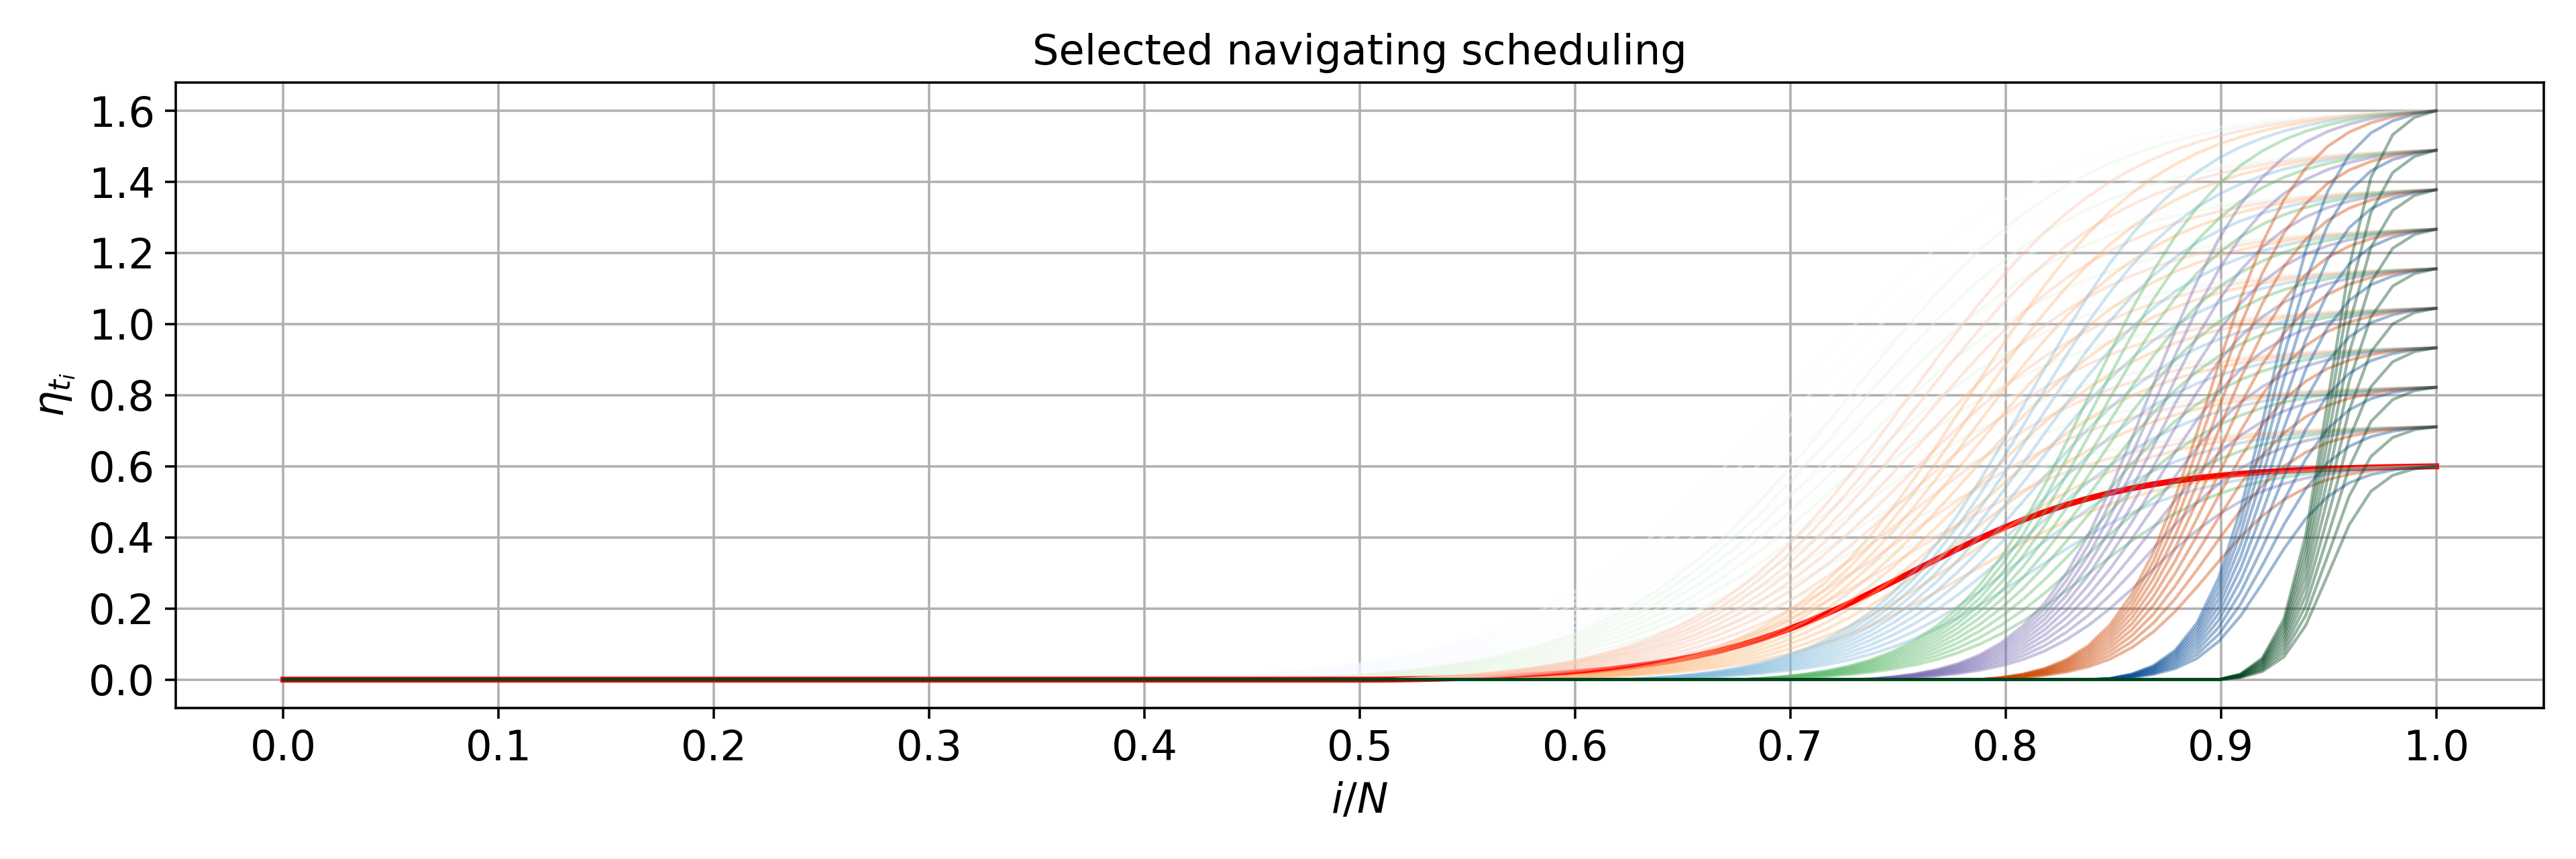
\includegraphics[width=0.75\linewidth]{images/figure-7.png}
    \caption{
        \textbf{Conformational dynamics of \flhac estimated by \Model}.
        \textbf{(a)} Distribution of the \acdii--\acdiv inter-domain distance estimated by \Model (red shaded) compared with AI-based structure generation models: AlphaFlow \cite{jing2024alphaflow}, BioEmu \cite{bioemu2025}, and \AFii with MSA subsampling \cite{delAlamo2022sampling}.
        \textbf{(b)} Time series of the six inter-domain distances estimated by \Model for the consecutive 159 experimental AFM frames.
        \textbf{(c)} Auto-correlation functions of the inter-domain distances as a function of time lag. Solid lines show the results from \Model estimations, while dashed lines correspond to temporally shuffled surrogate data.
    }
    \label{fig:flhac_statistic}
\end{figure}

\paragraph{Conformational dynamics}
To characterize the conformational dynamics captured by \Model, we computed the distribution of the \acdii--\acdiv inter-domain distance---a key indicator distinguishing between open and closed conformations---for all 159 estimated structures (\Cref{fig:flhac_statistic}~(a)).
For comparison, we also generated conformational ensembles using AI-based structure generation models: AlphaFlow \cite{jing2024alphaflow}, BioEmu \cite{bioemu2025}, and \AFii with MSA subsampling \cite{delAlamo2022sampling}, which are expected to approximate long-time behaviors of \flhac that are not accessible by brute-force MD simulations.
Interestingly, \Model tends to estimate more open conformational states than these AI-based models.
There are three possible explanations for this tendency.
First, HS-AFM captures molecular dynamics with a frame interval of 66~ms, which may reflect longer-timescale motions than those sampled by AlphaFlow or BioEmu, thereby enabling the observation of more open structures.
Second, interactions between the molecule and the stage during AFM imaging may stabilize conformations with larger contact surface areas, thus favoring more open structures.
Third, estimation errors in \Model could lead to an overrepresentation of highly open conformations with large conformational entropy.

To assess the third possibility, we examined the time series of the estimated inter-domain distances (\Cref{fig:flhac_statistic}~(b)).
Since the 159 AFM images are consecutive frames, we can expect temporal correlations in the estimated structures if the estimation errors are sufficiently small.
Indeed, the time series exhibits clear oscillatory behavior, with the distances fluctuating between larger (open) and smaller (closed) values over time.
Crucially, \Model estimates each frame independently without any temporal information, yet the estimated inter-domain distances display pronounced time correlations, implying that the estimation errors are smaller than the scale of the observed fluctuations.

This temporal correlation was quantified by the auto-correlation function (\Cref{fig:flhac_statistic}~(c)).
The auto-correlations from \Model estimations (solid lines) show a pronounced positive correlation for lag times up to 400~ms and oscillatory behavior at longer lag times.
In contrast, the auto-correlations from temporally shuffled surrogate data (dashed lines) remain low (within $\pm$0.2) across all lag times, confirming that the observed correlations are not artifacts of the estimation procedure.
Overall, these results demonstrate that \Model effectively captures conformational dynamics from the time series of HS-AFM images.

\section{Conclusion}

In this work, we have proposed a computational protocol, \Model, to predict the 3D conformation of biomolecules from AFM images. 
\Model extracts features from AFM images with a group-equivariant (symmetry-aware) CNN, reducing computational cost in two ways.
First, it reduces the amount of required training data, because symmetry-aware representations learn efficiently from limited images \cite{e2cnn}.
Second, it shortens inference time: guiding \AFiii requires computing $\ptc{\phi_{\text{object}}}{X_t}$; replacing this with $\mathcal{L}_{\text{MSE}}(X_t)$ keeps the computational cost per structure low.
In the estimations of this study, per-frame estimation finished within one minute on a single GPU.
It has the potential to serve as a useful tool for interpreting HS-AFM movies comprised of hundreds of frames in both structural and dynamic aspects.

A limitation of \Model is that it requires a priori definition of CVs as features to be estimated from the AFM image. If it is challenging to define appropriate CVs a priori, one could first perform structural sampling using methods such as AlphaFlow \cite{jing2024alphaflow}, BioEmu \cite{bioemu2025}, or \AFii with MSA subsampling \cite{delAlamo2022sampling}, and then identify meaningful CVs by applying dimensionality reduction techniques like PCA to extract important features. 
The \Model framework is general, and as long as the chosen CVs are differentiable with respect to atomic Cartesian coordinates and can be used for guiding \AFiii, a wide variety of CV types can be incorporated. For example, although we focused on inter-domain distances as CVs in this work, other CVs, such as residue-level distance restraints, can be used to enable AFM-guided reconstruction of finer-grained motions without a significant increase in computational cost.
The choice of CVs also determines the resolution at which structural degeneracy can be resolved.
As demonstrated in the \AK analysis (\Cref{fig:ak_cnn_training}~(d)), inter-domain distances alone cannot distinguish domain arrangements that differ in relative orientation (e.g., hinge-bending versus shear-like motions) but yield similar center-of-mass separations.
When the target protein exhibits such degenerate modes of motion, incorporating additional CVs---for example, inter-domain angles or residue-level distance restraints---would be necessary to lift the degeneracy and improve reconstruction fidelity.

Another limitation is that the g-CNN must be trained separately for each protein system, because the CVs and the training conformational ensemble are defined on a per-protein basis.
This per-protein preparation is not negligible: generating pseudo-AFM images for training takes some minutes, and training the g-CNN requires 2--3 days on a single GPU with 48~GB memory.
However, once trained, \Model estimates a conformation from each AFM image in approximately one minute, enabling rapid processing of tens to hundreds of frames.
More broadly, the per-protein setup of \Model currently involves several steps that require user decisions: the definition of CVs, the generation of training conformations via \AFiii, and the selection of guidance scheduling parameters.
Among these, the guidance scheduling was systematically evaluated in this work (see \Cref{sec:nav_scheduling}), and the results provide practical guidelines that can be reused across systems, reducing the need for exhaustive per-protein tuning.
The GPU hardware requirement (48~GB memory in this study) may also present a barrier for some experimental laboratories; however, cloud-based GPU services offer an increasingly accessible alternative.
These per-protein setup costs are one-time investments: once completed, the trained model can be applied to all frames of a given HS-AFM movie without further intervention.

It is also important to consider the intrinsic limitations of AFM imaging when interpreting the reconstructed structures.
First, each HS-AFM frame is acquired by raster scanning over a finite time (66~ms in the \flhac data set); if the molecule undergoes conformational changes during this interval, the resulting image represents a temporal average rather than an instantaneous snapshot, which could blur the distinction between neighboring conformational states.
Second, the lateral resolution is fundamentally limited by the convolution of the probe tip geometry with the molecular surface; as demonstrated in our robustness analysis (\Cref{fig:noise_robustness}~(e,f)), coarser resolution and larger tip radii degrade conformational discrimination.
For the \flhac data, the spatial resolution of $\sim$1.0~nm/pixel and estimated tip radius of 2--6~nm imply that sub-nanometer domain rearrangements may fall below the effective resolving power.
These factors set a practical lower bound on the conformational differences that \Model can reliably detect from experimental images and should be kept in mind when interpreting the modest numerical margins observed in the c.c.\ and embedding-distance comparisons (\Cref{fig:resnet_embeddings}~(b,c)).

More broadly, the reliance on simulated pseudo-AFM images for training introduces an inherent distribution mismatch with respect to real experimental data: the precise origins and statistics of experimental noise, tip--sample interactions, and imaging artifacts are difficult to reproduce exactly in simulation.
In this work, we adopted histogram matching as a simple and transparent adjustment, but achieving a fully realistic sim-to-real mapping remains an open challenge.
Future work could address this more systematically, for example by incorporating domain adaptation techniques that explicitly account for differences between simulated and experimental data distributions.

Another limitation of \Model is that it infers conformations from a single AFM image and currently does not quantify predictive uncertainty due to image noise or molecular orientation. 
Extending the framework to estimate uncertainty would make the predictions easier to interpret \cite{Kendall2017Uncertainty}.
Moreover, AFM image sequences constitute time-series data in which poses change only slightly between adjacent frames; incorporating temporal dependencies---for example, with TimeSformer \cite{Bertasius2021TimeSformer} or non-local networks \cite{Wang2018NonLocalNetworks}---could further improve fidelity.

Finally, in this work we navigated \AFiii's sampling only using AFM images; consequently, neither structural stability nor explicit physical priors are incorporated. 
In the future, conditioning the prior (such as Boltz-2's custom potentials \cite{passaro2025boltz2}) of an ensemble generative model should enable integrated modeling that unifies experimental measurements, physical priors, and computational inference. 

\input{sections/endmatter.tex}

% Uncomment if using biblatex
\sloppy
\printbibliography

% Uncomment if using bibtex
%\bibliography{citation_biophysj}

\section{Supplemental Material}

An online supplement to this article can be found by visiting BJ Online at \url{http://www.biophysj.org}.

\end{document}
